\documentclass[11pt,a4paper]{article}
\usepackage[margin=22mm,headheight=14pt]{geometry}
\usepackage{mathptmx,amsmath,amssymb,amsthm,booktabs,tabularx,array,graphicx,xcolor,float}
\usepackage[T1]{fontenc}
\usepackage{textcomp}
\renewcommand{\ttdefault}{pcr}
\usepackage{microtype,enumitem,caption,fancyhdr,placeins}
\usepackage[hidelinks]{hyperref}
\setlength{\parindent}{1.1em}
\setlength{\parskip}{2pt}
\renewcommand{\baselinestretch}{1.04}
\setlist{nosep,leftmargin=*}
\captionsetup{font=small,labelfont=bf}
\pagestyle{fancy}\fancyhf{}\fancyhead[L]{\small GPU discrete simulated bifurcation on a GH200}
\fancyfoot[C]{\thepage}\renewcommand{\headrulewidth}{0pt}
\newcommand{\blank}{\textcolor{gray}{---}}
\newcommand{\code}[1]{\texttt{#1}}
\newtheorem{proposition}{Proposition}
\graphicspath{{figures/}}
\title{GPU Discrete Simulated Bifurcation on a Grace Hopper Superchip:\\ Execution-Path Selection, Exact Low-Precision Arithmetic, and Scaling}
\author{Yaocheng Chen\\\small [Affiliation and corresponding author details to be completed]}
\date{}
\begin{document}
\maketitle\thispagestyle{plain}
\begin{abstract}
Simulated bifurcation (SB) solves Ising and quadratic unconstrained binary optimization problems by integrating a classical Hamiltonian system, and its discrete variant (dSB) reduces the dominant operation of each time step to a product of the coupling matrix with a sign vector. Here we present a CUDA implementation of dSB for the NVIDIA GH200 Grace Hopper Superchip that executes the same discrete dynamics through several execution paths---temporally fused persistent kernels that integrate all steps in one launch for dense, bit-packed (exclusive-or and population count) and compressed-sparse-row couplings, and cuBLAS products captured in a CUDA Graph with FP32, TF32, FP16 or INT8 operands---and evaluate all of them under one protocol on K2000, 16 G-set and 19 QPLIB instances. For couplings in $\{-1,0,+1\}$ we prove that the integer and bit-packed products are exact, and we verify that the TF32, FP32, INT8 and bit-packed paths return bitwise identical trajectories over 50 independent trials on every ternary instance, so their runtimes can be compared without a solution-quality confound. The fastest path is decided by the coupling density and the batch size: the fused CSR kernels are fastest on 27 of the 36 instances (all ten G-set instances up to an average degree of five and 17 of the 19 QPLIB instances), FP16 or INT8 tensor-core products on the denser ones at 512 replicas, and the fused bit-packed kernel on K2000 at 64 replicas or fewer (3.2~\textmu s per step at 16 replicas). Against the public \code{simulated-bifurcation} package run with a matched schedule, the fastest path is $13.6\times$ faster on K2000, $13.5$--$137\times$ on G-set and $18$--$86\times$ on QPLIB at equal work, while reaching the target at least as often on 35 of the 36 instances. The time to solution on K2000 (best-known cut 33337) is 0.20~s, below the 1.3~s of the single-FPGA dSB machine and the 1.7~s of the single-V100 dSB reported by Goto et al., and the coupling-product throughput of $1.65\times10^{5}$~GMAC/s is $88\times$ that of the 2048-spin FPGA design of Tatsumura et al. Sparse execution scales linearly to 200,000 vertices at $0.65\times10^{12}$ nonzero updates per second in 561~MB. Dense execution up to 240,000 variables runs at 86--88\% of the HBM3e bandwidth roofline, and by placing the coupling matrix in the coherent Grace memory the same path runs dense instances of 300,000 variables in FP32 and 450,000 in FP16 (360 and 405~GB), where the PyTorch baseline cannot allocate. Streaming the Grace-resident matrix through an HBM staging buffer sustains 371~GB/s over NVLink-C2C, 82\% of its nominal per-direction bandwidth, and keeping as many rows as fit in HBM while only the remainder is streamed (a hybrid placement) shortens the step by a further $1.4$--$3.7\times$, to 0.12--0.78~s, in agreement with an additive two-tier bandwidth model to within 4\%. A bit-packed path for dense $\pm1$ couplings applies the same placement on each of two GH200s connected by NVLink: at one bit per coupling it integrates dense instances of 3,000,000 variables (1.1~TB of couplings, 254~GB in HBM and 871~GB streamed from Grace memory) at 1.40~s per step, the two-tier model holding to within 2\%, and recovers the planted ground state of Mattis instances exactly at every size from 500,000 to 3,000,000 variables.
\end{abstract}
\noindent\textbf{Keywords:} discrete simulated bifurcation; GPU computing; Ising optimization; tensor cores; CUDA Graphs; time to solution.

\section{Introduction}
Quadratic unconstrained binary optimization (QUBO) and Ising models provide a common mathematical language for discrete optimization. Their expressive power allows problems with different application origins to be treated by the same solver infrastructure \cite{lucas,glover,boros}. This common representation has motivated both general-purpose software and specialized optimization machines. Simulated annealing is a foundational example of a stochastic search method \cite{kirkpatrick}, while simulated bifurcation (SB) approaches the same optimization task through the numerical evolution of classical dynamical variables \cite{goto2019,goto2021}.

The attraction of SB for parallel processors lies in its simultaneous variable updates. In discrete simulated bifurcation (dSB), the coupling force depends on the signs of the position variables. With multiple independent replicas, a dense step can be expressed as a matrix--matrix product followed by elementwise updates. This structure exposes substantial parallelism, but the cost of a complete trajectory also includes state movement, synchronization, and repeated submission of GPU work. An efficient matrix product alone therefore does not determine the performance of the complete solver.

Several execution strategies address different parts of this cost, and they do not have a fixed ranking. A persistent kernel integrates many steps while retaining replica states on chip, removing repeated launches and intermediate state traffic, but assigning one block to one replica leaves substantial duplication in the matrix loads requested by different blocks. Batched matrix multiplication exposes reuse across replicas through the library's tiles, but ordinarily launches new work at every step; a CUDA Graph removes the submission cost without removing the global intermediate traffic. Compressed sparse row storage removes the quadratic capacity requirement and, on sparse graphs, most of the arithmetic. Finally, a spin configuration is a one-bit quantity, and for couplings in $\{-1,0,+1\}$ the coupling product is an integer, so narrow arithmetic---INT8 tensor cores or bit-plane population counts---is not necessarily an approximation in this setting.

In this work, we present a CUDA implementation of dSB for a single NVIDIA GH200 that provides all of these paths for the same discrete dynamics (one of them also on two GH200s connected by NVLink), and we evaluate them under one protocol: the same instances, time steps, step budgets, replica counts and timing boundary for every path and for the external baseline. The evaluation asks where each path is the right one, how much of the measured speedup is arithmetic and how much is the removal of per-step host overhead, and whether runtime gains persist at a fixed solution target. The dSB dynamics themselves are unchanged throughout; no new algorithm is proposed. Our contributions are the following.
\begin{itemize}
\item We prove that the integer and bit-packed coupling products are exact for ternary couplings (Proposition~\ref{prop:exact}) and verify that the TF32, FP32, INT8 and bit-packed paths produce bitwise identical trajectories on every ternary instance in the benchmark set, which makes their runtime comparison free of any solution-quality confound.
\item We measure the region of the instance space in which each path is fastest---persistent CSR kernels up to average degree about five, tensor-core products above---and relate it to a data-movement and occupancy model that shows temporal fusion to be the decisive optimisation on sparse instances, where the fused CSR kernels are the fastest path on 27 of the 36 benchmark instances, and explains why the dense fused replica-tiled kernel is not competitive at the batch sizes used in SB benchmarks.
\item We compare against the public \code{simulated-bifurcation} package under a matched schedule and separately under its library defaults, and report integration time, objective distributions and time to solution for K2000, 16 G-set instances and 19 QPLIB instances, together with sparse and dense scaling families of up to 200,000 and 450,000 variables, the latter with the coupling matrix in HBM, in coherent Grace memory, or split between the two, a replica sweep on K2000 from 16 to 512 replicas, and a bit-packed dense $\pm1$ path that splits the coupling matrix over two GH200s and reaches 3,000,000 variables, with an exact correctness check on planted Mattis instances.
\item We place the results beside the published time-to-solution and throughput figures of FPGA and GPU SB machines on the shared instances, using the same definition of time to solution.
\end{itemize}
Quantities that the present campaign did not measure remain explicitly marked.

The rest of the paper is organized as follows. Section~\ref{sec:related} reviews related work. Section~\ref{sec:formulation} states the problem conventions and the discrete dynamics. Section~\ref{sec:paths} describes the execution paths and Section~\ref{sec:model} the performance model. Section~\ref{sec:method} gives the experimental methodology, including the alignment of the external baseline and the definition of time to solution. Section~\ref{sec:results} reports the results, Section~\ref{sec:discussion} discusses them, and Section~\ref{sec:conclusion} concludes.

\section{Related work}\label{sec:related}
\subsection{Simulated bifurcation and parallel optimization}
SB developed from the classical simulation of bifurcation dynamics associated with nonlinear oscillator models \cite{goto2016,goto2019}. Goto et al. subsequently introduced ballistic and discrete formulations that use bounded positions and permit simultaneous updates \cite{goto2021}. These formulations provide the algorithmic foundation of the present implementation. Kanao and Goto extended SB through thermal assistance \cite{kanao2022} and higher-order cost functions \cite{kanao2023}. More recent work explores tabu-enhanced trajectories \cite{tabu2026} and inter-replica interactions in simulated bifurcation quantum annealing \cite{sbqa2026}. Such approaches change the search dynamics. Independent GPU benchmarks by Zeng et al.\ find dSB to have the shortest time-to-target among the SB and simulated-coherent-Ising-machine variants on large dense graphs, including K2000 and G81 \cite{zeng2024}, and Tao et al.\ use a CUDA dSB implementation as the baseline for their tabu-enhanced variant \cite{tabu2026}; both adopt the time-to-solution convention of Goto et al.~\cite{goto2021}, which we also use (Section~\ref{sec:quality}). In the present study, replicas share coupling loads but do not exchange dynamical information, so implementation batching does not introduce an interaction among search trajectories.

Parallel SB has been implemented on FPGA hardware. Tatsumura et al.\ built 2048- and 4096-spin aSB machines on an Arria~10 FPGA with 8192 multiply--accumulate units, reaching 1.9--2.0~TMAC/s, and reported a single-V100 implementation of the same algorithm at 0.11--0.18~TMAC/s, bound by the HBM2 bandwidth because the coupling matrix is re-read at every step \cite{fpga2019}. Goto et al.\ implemented bSB and dSB machines on a Stratix~10 FPGA and on a V100 and benchmarked them by time to solution on K2000 and the G-set \cite{goto2021}; the FPGA line has since been extended to multi-chip architectures \cite{tatsumura2021} and to real-time systems \cite{tatsumura2021heart}. These studies establish the relevance of mapping coupling evaluation and state updates onto hardware with explicit communication and memory constraints, and they supply the published figures against which Section~\ref{sec:res-literature} places the present results. Simulated bifurcation is one member of a broader family of physics-inspired and hardware-assisted Ising solvers surveyed by Mohseni et al.~\cite{mohseni2022}, which includes digital annealers with application-specific update rules \cite{aramon2019} and GPU realisations of oscillator-based Ising and Potts machines \cite{gonul2025} and of digital annealing for large instances \cite{vamsi2025}. These systems differ in their update rule and therefore in their search dynamics; they are relevant here as context for what a general-purpose GPU is being asked to do, not as algorithmic components of the present implementation. Our target is a single GPU with several execution paths for the same quadratic dynamics, plus a two-GPU extension of one path for very large dense $\pm1$ instances. The public \code{simulated-bifurcation} package supplies a practical external baseline \cite{publicsb} built on PyTorch \cite{pytorch}. We distinguish comparisons against its default package behavior from schedule-aligned measurements, because initialization, schedules, stopping rules, and numerical settings can affect both runtime and solution quality.

Preprocessing by Hamiltonian reduction, such as FastHare \cite{fasthare} and its general-order extension \cite{mao2026}, is complementary to the execution paths studied here: it changes the instance before the solver runs. The implementation retains an interface to the original FastHare reducer, but no reduced instance is used in the present evaluation; every result below is obtained on the original standardized instance.

\subsection{GPU execution and performance assessment}
Efficient GPU linear algebra depends on the balance between data movement and arithmetic. The Roofline model provides a useful framework for interpreting this balance \cite{roofline}. Dense batching can increase coupling reuse, while sparse multiplication requires attention to row structure and irregular memory access \cite{bell2009}; Yang et al.\ analyse the design space for sparse matrix products on GPUs and the conditions under which a row-oriented schedule is preferable \cite{yang2018}. CUDA Graphs reduce repeated submission overhead, cuBLAS provides optimized dense matrix products, and Hopper shared-memory features determine the feasible persistent state size \cite{cuda,cublas,hopper}. We use these mechanisms within the dSB trajectory and evaluate their interaction, rather than regard their use alone as an algorithmic contribution.

Optimization benchmarks require a distinction between computational throughput and the probability of reaching a target. R\o nnow et al. discuss how benchmark definitions affect speedup claims \cite{ronnow}, while optimized simulated-annealing implementations illustrate the importance of strong classical baselines \cite{isakov2015}. Performance profiles provide a complementary way to summarize relative behavior across heterogeneous instances \cite{dolan2002}, systematic comparisons of Max-Cut and QUBO heuristics show how strongly reported rankings depend on budget and instance family \cite{dunning2018}, and strong local-search references such as breakout local search remain competitive on the G-set instances \cite{benlic2013}. We cite these to delimit the claim made here: the present comparison is against a public dSB package under matched work, not a claim of superiority over the Max-Cut heuristic literature.

\subsection{Reduced precision and bit-level arithmetic on GPUs}
Tensor cores expose matrix-multiply pipelines whose operand format is narrower than the accumulator. Their programmability and numerical behaviour were characterised early by Markidis et al.~\cite{markidis2018}, and Haidar et al.\ demonstrated that a narrow operand format can be used in a scientific solver without loss of final accuracy when the surrounding algorithm controls the error \cite{haidar2018}. The Hopper generation extends this range with additional operand formats and distributed shared memory; Luo et al.\ report a detailed characterisation of the resulting instruction and memory behaviour \cite{luo2024}.

At the extreme of this progression, one-bit operands are executed through logical operations and population counts. Li et al.\ describe bit-level tensor-core execution for binarised networks and the associated data layout \cite{li2019bstc,li2021bittc}. The relevance to Ising dynamics is direct but has a different character than in machine learning: a spin configuration is already a one-bit quantity, and for couplings restricted to $\{-1,0,+1\}$ the coupling product is an integer. Narrow arithmetic is therefore not necessarily an approximation in this setting, which distinguishes the present use from quantisation as an accuracy trade-off. Section~\ref{sec:bitexact} states the condition under which the integer and bit-packed paths are exact.

\subsection{Tightly coupled CPU--GPU platforms}
The target platform couples a Grace CPU and a Hopper GPU over a coherent NVLink-C2C link, so host memory is addressable by the GPU at a bandwidth between HBM and a PCIe-attached host. Early scientific-workload assessments of this configuration are given by Simakov et al.~\cite{simakov2024}, and the consistency and coherence behaviour of the link has been examined separately \cite{bagchi2026}. For dense dSB the relevant consequence is a capacity hierarchy rather than a change in kernel design: the coupling matrix may reside in HBM, spill entirely into coherent host memory at reduced bandwidth, or be split between the two. Section~\ref{sec:placement} describes these placements and Section~\ref{sec:capacity} treats the resulting dimension limits and step times as explicit functions of the bytes used per coupling.

\section{Problem formulation and discrete dynamics}\label{sec:formulation}
\subsection{Ising and Max-Cut conventions}
We use the minimization convention
\begin{equation}
 E(\boldsymbol{s})=-\tfrac12\boldsymbol{s}^{\mathsf T}J\boldsymbol{s}
 -\boldsymbol{h}^{\mathsf T}\boldsymbol{s}+c,\qquad s_i\in\{-1,+1\},
 \label{eq:ising}
\end{equation}
where $J$ is symmetric and has zero diagonal. A diagonal contribution is constant for binary spins and must be moved into $c$. For an undirected weighted graph, the cut objective is
\begin{equation}
 C(\boldsymbol{s})=\tfrac12\sum_{(i,j)\in\mathcal E}w_{ij}(1-s_i s_j).
 \label{eq:cut}
\end{equation}
Choosing $J_{ij}=-w_{ij}$ makes energy minimization equivalent to cut maximization. Each undirected edge occurs once in Eq.~\eqref{eq:cut} and twice in the symmetric matrix. Sign and factor-of-two conventions are verified before transferring a problem between software packages.

For a symmetric QUBO $f(\boldsymbol{z})=\boldsymbol{z}^{\mathsf T}Q\boldsymbol{z}+\boldsymbol{a}^{\mathsf T}\boldsymbol{z}+c_0$, substitute $\boldsymbol{z}=(\boldsymbol{1}+\boldsymbol{s})/2$. The spin-dependent terms are $\boldsymbol{s}^{\mathsf T}Q\boldsymbol{s}/4+(Q\boldsymbol{1}+\boldsymbol{a})^{\mathsf T}\boldsymbol{s}/2$. This identity defines the mathematical conversion; a file containing triangular coefficients or a prefactor of one half requires its own parsing convention. General constrained quadratic programs are outside the present solver scope unless separately transformed and validated. We therefore restrict QPLIB experiments to an explicitly checked compatible subset \cite{qplib}.

\subsection{Integration step}\label{sec:step}
Let $X,Y\in\mathbb R^{n\times B}$ denote positions and momenta of $B$ replicas. A field-free trajectory uses $S_k=\operatorname{sgn}(X_k)$ and
\begin{align}
 A_k &= J S_k,\label{eq:coupling}\\
 Y_{k+1} &=Y_k+\Delta t[-(\delta-p_k)X_k+\xi A_k],\\
 \widetilde X_{k+1}&=X_k+\Delta t\,\delta Y_{k+1}.\label{eq:update}
\end{align}
If $|\widetilde x_{ib}|>1$, the implementation sets $x_{ib}=\operatorname{sgn}(\widetilde x_{ib})$ and $y_{ib}=0$; otherwise it retains the updated values. Signs are computed from the old positions for every row before the next state is exposed. The integration convention has $\operatorname{sgn}(0)=0$; returned solutions must be checked to contain only binary spins, with any zero-resolution policy applied consistently before scoring.

The schedule is $p_k=k/(K-1)$ for $K>1$ and $p_0=0$ for $K=1$, with $\delta=1$ and
\begin{equation}
 \xi=\frac{0.5\sqrt{n-1}}{\|J\|_F}
 \label{eq:gain}
\end{equation}
when $\|J\|_F>0$; a zero matrix uses $\xi=0$. Initial positions and momenta are sampled uniformly in $(-0.01,0.01)$. The time step is chosen per instance: the discrete dynamics diverge when $\Delta t^2\,\xi\,|\lambda_{\min}(J)|$ exceeds roughly $2.7$, after which all spins collapse to one side and the cut approaches zero, so we set $\Delta t=\operatorname{clip}(\sqrt{1.2/(\xi|\lambda_{\min}(J)|)},\,0.25,\,1.25)$ from a sparse eigenvalue estimate of $\lambda_{\min}(J)$. The resulting values range from $0.50$ on the dense G-set instances (average degree 12--48) to $1.10$--$1.18$ on K2000 and the 4-regular instances, and the same value is passed to the public baseline (Section~\ref{sec:align}). Equations~\eqref{eq:coupling}--\eqref{eq:update} are the dSB update of Goto et al.~\cite{goto2021} with $a_0=\delta$, $a(t_k)=p_k$ and $c_0=\xi$; Eq.~\eqref{eq:gain} is their choice $c_0=0.5/(\langle J\rangle\sqrt n)$ with $\langle J\rangle$ the root-mean-square off-diagonal coupling, and $K$ and $B$ are their $N_{\mathrm{step}}$ and $N_{\mathrm{batch}}$. We keep $K$ and $B$ in the text because they are also the launch parameters of the kernels. Equality of $B$, $K$, and storage precision does not by itself establish equality with a public solver: its schedule, gain, initialization, update ordering, and stopping rule must also be recorded.

\subsection{Field absorption and standardization}\label{sec:lifting}
A linear field can be absorbed using an auxiliary spin $s_a$ and an augmented matrix with $\bar J_{ia}=h_i$. The augmented energy is invariant under simultaneous reversal of all spins. After solving, the original variables are recovered as $s_i=\bar s_i\bar s_a$. This gauge correction is applied before any objective is evaluated or any two implementations are compared. All final objectives are recomputed from the original instance on the host after gauge correction, so a reported cut never depends on a constant or a scaling used inside the solver. Both implementations under comparison start from the same standardized problem, including its normalization and auxiliary spin.

\subsection{Numerical structure of the update}\label{sec:numstruct}
Three structural properties of Eqs.~\eqref{eq:coupling}--\eqref{eq:update} determine where numerical format can and cannot affect the trajectory, and they are used later to justify comparing execution paths without a quality confound.

First, the coupling term depends on $X_k$ only through $S_k=\operatorname{sgn}(X_k)$. The dynamical state is continuous, but the quantity entering the matrix product is one bit per variable per replica. Any storage format that represents $\{-1,+1\}$ exactly, which includes FP32, FP16, BF16, TF32, INT8 and a one-bit packing, introduces no error on the right-hand operand. Error in $A_k$ can therefore originate only in the representation of $J$ and in the arithmetic of the product itself.

Second, the map from $(X_k,Y_k,A_k)$ to $(X_{k+1},Y_{k+1})$ is deterministic and contains no reduction across replicas. Replicas interact only through shared reads of $J$. Consequently two configurations that agree on the initial state and on $A_k$ at every step, and that evaluate the elementwise update in the same floating-point order, agree on the entire trajectory, exactly and not merely in distribution. This is the induction used in Section~\ref{sec:bitexact}, and it is what makes bitwise agreement a meaningful validation target rather than an unreachable ideal for a chaotic system.

Third, the clipping rule, which sets $x_{ib}=\operatorname{sgn}(\tilde x_{ib})$ and $y_{ib}=0$ when $|\tilde x_{ib}|>1$, is a discontinuous function of the state. Near the threshold an arbitrarily small numerical difference can change a sign and thereafter a trajectory. This is the reason a path that is not bitwise identical cannot be validated by a tolerance on the final state of a long trajectory and is instead compared through objective distributions over independent trials, and the reason the tolerance-based checks of Table~\ref{tab:validation} are applied to short trajectories where divergence has not yet had time to develop.

\section{GPU execution paths}\label{sec:paths}
All paths integrate the same Eqs.~\eqref{eq:coupling}--\eqref{eq:update} with FP32 dynamical state and differ only in how $A_k=JS_k$ is evaluated and where the state resides. Four of them---the dense \code{block} kernel, the bit-packed \code{bit} kernel and the two CSR kernels---are temporally fused: one persistent kernel launch integrates all $K$ steps, with steps separated by in-kernel barriers rather than by host launches. The \code{gemm} path is not fused; it removes the per-step host submission with a CUDA Graph instead.

\subsection{Dense fused kernel with replica reuse}\label{sec:fused}
The dense \code{block} path assigns one thread block to one replica and executes all $K$ steps within one kernel. Position and momentum use FP32 shared memory, while signs use signed bytes, giving a state footprint of approximately $9n$ bytes. The coupling matrix remains in device memory and is streamed from L2 or HBM once per step per block. Temporal fusion removes repeated host launches and intermediate global-memory state updates; it does not hold the entire dense matrix on chip.

The \code{block-tiled} extension assigns $R\in\{1,2,4,8\}$ replicas to one block. A warp processes a coupling row in column segments and each loaded coefficient contributes to $R$ accumulators, using the signs of the corresponding replicas, so that matrix reuse is achieved inside the dot product rather than by replicating the matrix in shared memory. Position, momentum, accumulator and sign storage require
\begin{equation}
 M_{\mathrm{shared}}\simeq (4+4+4+1)nR=13nR\ \mathrm{bytes},
 \label{eq:shared}
\end{equation}
so at $n=2000$, $R=4$ needs 104,000 bytes and $R=8$ needs 208,000 bytes against the 232,448-byte opt-in limit of the device. The block count is $\lceil B/R\rceil$; increasing $R$ trades matrix reuse against the number of resident blocks. Section~\ref{sec:occupancy} shows that at the batch sizes used in this study the second constraint forces $R=1$, so the measurements below use the \code{block} path and the replica-tiled variant is characterised analytically only.

\subsection{Graph-based dense matrix multiplication}\label{sec:graphgemm}
The \code{gemm} path represents the signs of all replicas as an $n\times B$ matrix and evaluates $A=JS$ with cuBLAS. One update kernel modifies positions and momenta, clips the states, and writes the signs required by the next multiplication. Stream capture records the initial sign kernel followed by $K$ GEMM/update pairs; at the API-operation level this is $1+2K$ operations, although a cuBLAS operation can expand into multiple internal graph nodes. Graph execution reduces repeated host submission; it does not fuse the matrix products into a single kernel or eliminate their global-memory traffic.

The graph is prepared before the integration CUDA events. Its cache depends on the step count, buffer addresses, pump pointer, and dynamical parameters; matrix dimension, batch size, and math mode belong to the stepper object, so changing them requires rebuilding the graph or constructing another solver. A cuBLAS workspace is allocated before capture, and capture failures produce an error rather than an assumed fallback to an uncaptured loop.

The \code{gemm} path is run in four math modes with the same FP32 state: FP32 operands with TF32 tensor-core multiplication (the cuBLAS default on Hopper, labelled \code{gemm} TF32), FP32 operands with the tensor cores disabled (\code{gemm} FP32), FP16 operands with FP32 accumulation (\code{gemm} FP16), and INT8 operands with INT32 accumulation (\code{gemm} INT8). Two observations delimit the numerical consequence. First, the right-hand operand $S_k$ has entries in $\{-1,+1\}$ and is represented exactly in every one of these formats, so no error is introduced on the state side. Second, for integer-weighted instances a coupling of magnitude at most $w_{\max}$ is representable exactly in FP16 and in TF32 (both have an 11-bit significand) whenever $w_{\max}\le 2048$, so on the G-set, K2000 and ternary QPLIB families every math mode stores $J$ without loss; whether the products are also exact is the subject of Section~\ref{sec:bitexact}.

\subsection{Dense matrix placement beyond HBM}\label{sec:placement}
For dense instances whose coupling matrix does not fit in HBM, the \code{gemm} path places the matrix in one of three ways. In \emph{HBM placement} the matrix is an ordinary device allocation; it is selected while matrix and state fit within 0.85 of the free device memory. In \emph{Grace placement} the whole matrix resides in the LPDDR5X memory of the Grace CPU. The solver reserves it with an anonymous memory map bound to the NUMA node local to the GPU and pins it with \code{cudaHostRegister}, so that its pages are neither migrated nor duplicated into HBM; it is deliberately not allocated as driver-managed memory, because the driver's page migration turns a streaming pass over a matrix larger than HBM into fault-driven copies. The matrix is generated in place by a GPU kernel writing over NVLink-C2C. During integration the Grace-resident rows are not read in place by cuBLAS: every step copies them, in blocks of rows, into a 2~GiB HBM staging buffer with \code{cudaMemcpyAsync} and multiplies each block from there, and the copies are captured in the same CUDA Graph as the products and the update kernels. Because row $i$ of $J$ is column $i$ of the transposed product, a block of rows of $J$ produces a disjoint block of the output and the partial products need no reduction. In \emph{hybrid placement} the first $R$ rows are allocated in HBM, with $R$ chosen so that they, the state, the GEMM buffers and the staging block fill the HBM budget, and only the remaining $n-R$ rows are placed in Grace memory as above; each step issues one product over the HBM rows followed by the staged products over the Grace rows. Copies and products share one stream, so a copy waits for the product that reads the previous block; the two are not overlapped. All three placements run the same update kernel on the same state, and the dense generator depends only on the global row and column index, so the coupling values are identical in every placement. The dense $\pm1$ bit path of Section~\ref{sec:bitexact} uses the same three placements on each GPU, with the rows of the matrix divided between one or two GH200s.

\subsection{Sparse execution}\label{sec:sparse}
Sparse couplings use CSR arrays with row pointers, column indices, and FP32 values, following the standard sparse linear-algebra representation \cite{bell2009}. For an undirected graph stored symmetrically, $\mathrm{nnz}=2|\mathcal E|$. Both CSR paths are fused in the same sense as \code{block}: a single persistent kernel integrates all $K$ steps, so that no step is launched from the host and the per-step cost is the sparse product plus one barrier. The \code{csr-row} path assigns one block to each coupling row, with threads covering the replicas, and synchronises the whole grid once per step with a cooperative-groups barrier; the state lives in device memory, so it scales to any $n$ that fits in memory and is the path used for the large sparse graphs of Section~\ref{sec:res-sparse}. The \code{csr-block} path assigns one persistent block to each replica, with one thread per row, and needs no grid-wide synchronisation because a replica's state is private to its block; each block re-reads the CSR arrays every step, so it is fastest when they fit in L2 and the average degree is low. The implementation contains four further variants that are not compared in the rest of the paper; all appear in the K2000 panorama of Section~\ref{sec:res-k2000}, none was competitive there, and they were therefore not run on the G-set and QPLIB suites. The \code{global-sync} path keeps the state in device memory and synchronises the whole grid once per step; it is a diagnostic reference and the slowest dense path (9.2~ms per step on K2000 at $B=512$), because every step pays a grid-wide barrier and a round trip of the state through global memory without any replica reuse. The \code{cluster} and \code{csr-cluster} variants split one replica over a Hopper thread-block cluster through distributed shared memory \cite{hopper}; they are intended for dimensions that one block cannot hold, and at the benchmarked sizes the cluster barrier and the shared-memory exchange add cost without adding reuse (2.1 and 9.8~ms per step on K2000). FP16 storage in the fused kernel halves the coupling bytes but shortens the \code{block} step only from 0.77 to 0.65~ms, since that step is limited by occupancy rather than by bandwidth (Section~\ref{sec:occupancy}).

\subsection{Bit-packed and integer execution}\label{sec:bitexact}
Two further paths exploit the fact that a spin vector is a one-bit quantity. The \code{gemm} INT8 path issues the coupling product on the integer tensor-core pipeline with INT32 accumulation. The \code{bit} path is a fused persistent kernel that stores the coupling matrix as bit planes in shared memory together with the replica state for the whole trajectory and evaluates each row through exclusive-or and population count, with a dense $\pm1$ form using one plane and a sparse ternary form using a magnitude plane and a sign plane. Both paths require couplings drawn from $\{-1,0,+1\}$, which covers unweighted Max-Cut, the K2000 family, and the QPLIB instances whose quadratic coefficients are uniform after scaling.

\begin{proposition}
\label{prop:exact}
Let $J\in\{-1,0,+1\}^{n\times n}$ and $S\in\{-1,+1\}^{n\times B}$, and let $A=JS$. Then every entry of $A$ is an integer with $|A_{ib}|\le n$, and:
\begin{enumerate}
\item[(i)] an INT8 product with INT32 accumulation returns $A$ exactly whenever $n<2^{31}$;
\item[(ii)] any floating-point product whose operands represent $J$ and $S$ exactly and whose accumulator has at least $\lceil\log_2 n\rceil+1$ significand bits returns $A$ exactly, in any summation order; with FP32 accumulation this holds for $n<2^{24}$, and it holds for TF32, FP16 and BF16 operands as well as FP32 operands;
\item[(iii)] if $J$ has no zero entries, write $J_{ij}=1-2u_{ij}$ and $S_{jb}=1-2v_{jb}$ with $u,v\in\{0,1\}$; then $A_{ib}=n-2\,\mathrm{popcount}\!\left(u_i\oplus v_b\right)$;
\item[(iv)] in general, let $m_{ij}=\mathbf{1}[J_{ij}\neq 0]$; then $A_{ib}=\mathrm{popcount}(m_i)-2\,\mathrm{popcount}\!\left(m_i\wedge(u_i\oplus v_b)\right)$, where $u$ encodes the sign of the nonzeros.
\end{enumerate}
\end{proposition}

\begin{proof}
Each term $J_{ij}S_{jb}$ lies in $\{-1,0,+1\}$, so $A_{ib}$ is an integer bounded by the row support, hence by $n$; INT32 accumulation is exact under that bound, giving (i). For (ii), every partial sum is an integer of magnitude at most $n$, and every integer of magnitude below $2^{p}$ is representable exactly in a floating-point format with $p$ significand bits, so no rounding occurs at any step of the summation regardless of its order. For (iii), $J_{ij}S_{jb}=+1$ exactly when $u_{ij}=v_{jb}$, so the number of $+1$ terms is $n-\mathrm{popcount}(u_i\oplus v_b)$ and the number of $-1$ terms is $\mathrm{popcount}(u_i\oplus v_b)$; subtracting gives the stated identity. For (iv) the same count is taken over the support selected by $m_i$.
\end{proof}

Proposition~\ref{prop:exact} has a methodological consequence that is used throughout Section~\ref{sec:results}. The integration step is a deterministic function of $(X_k,Y_k,A_k)$. If two configurations start from identical states, produce identical $A_k$ at every step and apply the elementwise update in the same floating-point order, their trajectories coincide exactly, not merely in distribution. On ternary instances the dense FP32, TF32, INT8 and bit-packed paths, which share one update kernel, therefore return bitwise identical spin sequences, and any runtime difference between them is attributable to execution alone, with no quality confound. This removes, for that instance class, the usual objection that a faster configuration may simply be searching differently. Part~(ii) implies that a product with FP16 operands and FP32 accumulation would also be exact; the \code{gemm} FP16 path of our implementation is nevertheless not bitwise identical to the FP32 paths (Section~\ref{sec:res-identity}), which shows that its product is not formed as the pure integer sum assumed in (ii), for example because the coupling gain is applied before the conversion to FP16; the cause was not isolated in this study and the path is compared empirically. The CSR paths evaluate the elementwise update in a different kernel and are likewise compared empirically.

The bit-packed path also changes the storage cost per coupling from four bytes to one eighth of a byte in the dense $\pm1$ form and one quarter of a byte in the ternary form. In the benchmark kernel the bit planes and the state of a replica tile reside in shared memory, which bounds $n$ by the per-block shared-memory limit: at $B=512$ the planner reports that the path does not fit for $n\ge 3000$ (it requests 509,056 bytes per block at $n=5000$), so \code{bit} results on the benchmark suites exist only for $n\le 2000$.

To use the storage advantage where it matters, the dense $\pm1$ form has a second implementation, the program \code{bit\_dense\_multi}, which keeps the packed matrix in device memory instead of shared memory and integrates one replica. Each row is stored as one bit per coupling (bit~1 for $+1$; the diagonal is stored as $+1$ and removed in the product), padded to a multiple of 128 bits. The rows are divided between one or two GH200s, and on each GPU the first rows are placed in HBM and the remaining rows in pinned Grace memory on that GPU's own NUMA node, staged through a 2~GiB HBM buffer at every step exactly as in the hybrid placement of Section~\ref{sec:placement}. A warp evaluates four rows against the sign bitmap with 128-bit loads, exclusive-or and population count, so the product is the integer identity of Proposition~\ref{prop:exact}(iii); the update kernel writes the new signs of its rows into a bitmap, and after each step the two GPUs exchange their $n/8$-byte bitmap segments over NVLink with peer-to-peer copies, which is the only inter-GPU traffic. The update is compiled without fused multiply--add contraction and uses explicit round-to-nearest intrinsics, so the trajectory does not depend on the number of GPUs or on the placement; at $n=8192$ and $K=100$ the final state was compared bit for bit with a host reference on one GPU, on two GPUs, and on two GPUs with all but 1024 rows per GPU forced into Grace memory, and all three runs matched it with identical checksums. The same program generates Mattis instances $J_{ij}=\xi_i\xi_j$ from a hidden random $\xi\in\{\pm1\}^n$, whose ground states $s=\pm\xi$ have energy $-n(n-1)/2$, so that a run at any size reports whether the planted optimum was reached (Section~\ref{sec:res-bitmulti}).

\subsection{Summary of execution paths}
\begin{table}[!ht]\centering\small
\caption{Execution paths evaluated. Bytes per coupling are storage costs for the coupling matrix only. ``Exact on ternary'' is the prediction of Proposition~\ref{prop:exact} for a path that shares the FP32 update kernel; the measured outcome is in Section~\ref{sec:res-identity}. $B$ is the number of replicas.}
\label{tab:paths}
\begin{tabularx}{\linewidth}{lXccc}\toprule
Path & Coupling evaluation & Bytes/coupling & State location & Exact on ternary \\
\midrule
\code{block}       & FP32 row dot product, fused, one block per replica     & 4     & shared memory   & yes \\
\code{gemm} TF32   & cuBLAS, TF32 tensor cores, FP32 accumulate             & 4     & device memory   & yes \\
\code{gemm} FP32   & cuBLAS, FFMA (tensor cores disabled)                   & 4     & device memory   & yes \\
\code{gemm} FP16   & cuBLAS, FP16 operands                                  & 2     & device memory   & no (measured) \\
\code{gemm} INT8   & cuBLAS, INT8 operands, INT32 accumulate                & 1     & device memory   & yes \\
\code{bit}         & fused; XOR/popcount over packed planes in shared memory & $1/8$--$1/4$ & shared memory & yes \\
\code{bit\_dense\_multi} & XOR/popcount over one packed plane in HBM and Grace memory, rows split over 1--2 GPUs, $B=1$ & $1/8$ & device memory & yes \\
\code{csr-row}     & fused; FP32 CSR, one block per row, grid barrier per step & $\approx 8$/nnz & device memory & separate update kernel \\
\code{csr-block}   & fused; FP32 CSR, one persistent block per replica & $\approx 8$/nnz & device memory & separate update kernel \\
\bottomrule
\end{tabularx}
\end{table}

\section{Performance model}\label{sec:model}
\subsection{Work and data movement}
Ignoring lower-order updates, dense dSB performs approximately $2Kn^2B$ floating-point operations. A one-replica matrix-streaming model loads $4Kn^2B$ bytes of FP32 coupling data, about $0.5$ operations per coupling byte. Let $b$ denote the bytes stored per coupling and $\rho$ the achieved replica reuse depth, that is, the number of replicas served by one load of a coupling coefficient. The idealised coupling traffic and intensity are
\begin{equation}
 Q_J\simeq b\,Kn^2\lceil B/\rho\rceil,\qquad
 I\simeq\frac{2B}{b\lceil B/\rho\rceil}\approx\frac{2\rho}{b}.
 \label{eq:intensity}
\end{equation}
For the fused paths $\rho$ equals the replica tile $R$ ($R=1$ for \code{block}); for the library path $\rho=\min(B,\beta)$, where $\beta$ is the extent of the selected kernel's tile along the replica dimension, a property of the library that we do not control. The model counts coupling loads requested by the algorithm, not measured HBM transactions: L2 hits can make physical traffic smaller, while poor occupancy or imperfect access can make the runtime prediction inaccurate. Sign traffic, reductions, barriers, and shared-memory accesses remain outside $I$. An illustrative decomposition of the step time is
\begin{equation}
 T_{\mathrm{dense}}\approx T_{\mathrm{dispatch}}+
 \max(F/P_{\mathrm{eff}},Q/BW_{\mathrm{eff}})+T_{\mathrm{sync}},
 \label{eq:tdense}
\end{equation}
where effective compute rate and bandwidth refer to the particular kernel. This expression is explanatory rather than a calibrated predictor. For the sparse paths the work is $\propto K B\,\mathrm{nnz}$ and the coupling traffic $\propto K\,\mathrm{nnz}\lceil B/\rho\rceil$, with $\rho=B$ for \code{csr-row} (one load of a row serves every replica) and $\rho=1$ for \code{csr-block} (every block re-reads the CSR arrays).

\subsection{Replica reuse and occupancy}\label{sec:occupancy}
Equation~\eqref{eq:shared} bounds the replica tile of the fused path by the per-block shared-memory budget $S_{\max}$,
\begin{equation}
 R_{\max}(n)=\left\lfloor \frac{S_{\max}}{13n} \right\rfloor .
 \label{eq:rmax}
\end{equation}
It is not the only bound. The fused path launches $\lceil B/R\rceil$ blocks, and each block occupies one streaming multiprocessor for the duration of the trajectory because its state is resident. On a device with $N_{\mathrm{SM}}$ multiprocessors, filling the machine requires $\lceil B/R\rceil\ge N_{\mathrm{SM}}$, that is $R\lesssim B/N_{\mathrm{SM}}$. Reuse and parallelism are therefore in direct competition, and the effective tile is
\begin{equation}
 R_{\mathrm{eff}}=\min\!\left(\left\lfloor \frac{S_{\max}}{13n} \right\rfloor,\ \left\lfloor \frac{B}{N_{\mathrm{SM}}} \right\rfloor \right).
 \label{eq:reff}
\end{equation}
Substituting into Eq.~\eqref{eq:intensity}, the fused path has the lower coupling traffic than the library path when $R_{\mathrm{eff}}/b_{\mathrm{fused}} > \min(B,\beta)/b_{\mathrm{gemm}}$.

On the device used here, $N_{\mathrm{SM}}=132$ and $S_{\max}=232{,}448$ bytes. At $n=2000$, Eq.~\eqref{eq:rmax} admits $R_{\max}=8$, but at $B=512$ the occupancy bound admits only $R\le 3$, and at $B=200$ only $R\le 1$; obtaining $R=8$ together with full occupancy requires $B\ge 1056$. Reuse and occupancy can be obtained simultaneously only in a large-batch regime, and at the batch sizes at which SB benchmarks are usually reported the dense fused path retains its launch and state-traffic advantages but loses most or all of its matrix-reuse advantage. This is why the measurements in Section~\ref{sec:results} use the fused path with $R=1$ and why it is an order of magnitude slower than the library path on K2000: the comparison is taken at a batch size that places the dense fused kernel outside its own design regime. The two effects saturate at different points---$\beta$ for the library path and $S_{\max}/13n$ for the fused path---so the ordering is not monotone in $B$ and cannot be inferred from a single batch size; probing the boundary predicted here requires $B\ge 1056$ and is left for future work.

\subsection{Storage format and dense capacity}\label{sec:capacity}
A dense coupling matrix at $b$ bytes per coupling occupies $bn^2$, so the largest dimension admitted by a memory budget $M$ is $n_{\max}=\sqrt{M/b}$ before state arrays, padding and workspace. Table~\ref{tab:capacity} gives these analytic limits for the storage formats of Table~\ref{tab:paths} at two budgets: the 0.85 fraction of HBM that the implementation allows the coupling matrix to occupy, and a budget that includes the 480~GB of coherent host memory reachable over NVLink-C2C. The second column is a capacity statement, not a performance statement, because host-resident pages are served at lower bandwidth. The measured columns record the largest dimension that was actually run in the dense sweep of Section~\ref{sec:res-dense}, which used the \code{gemm} path with FP32 and FP16 storage, with the coupling matrix in HBM and, when it no longer fits there, in Grace memory or split between HBM and Grace memory (Section~\ref{sec:placement}), together with the largest dimension the PyTorch baseline could allocate; the INT8 and ternary bit-packed rows are analytic only, because the dense-capacity generator produces real-valued couplings and the benchmark \code{bit} kernel keeps its planes in shared memory (Section~\ref{sec:bitexact}); the dense $\pm1$ row is measured with \code{bit\_dense\_multi} on two GH200s (Section~\ref{sec:res-bitmulti}), whose combined budget is twice that of the column headings.

Capacity and speed are linked through the same roofline. A dense step reads the whole coupling matrix once, so if $M_H$ bytes of it reside in HBM and $M_G=bn^2-M_H$ bytes are streamed from Grace memory, the step time is approximately
\begin{equation}
 T_{\mathrm{step}}\approx \frac{M_H}{BW_H}+\frac{M_G}{BW_G},
 \label{eq:tier}
\end{equation}
with $BW_H$ and $BW_G$ the bandwidths at which the two memories deliver the matrix to the product. HBM placement is the case $M_G=0$ and Grace placement the case $M_H=0$; hybrid placement fixes $M_H$ at the HBM budget, so its advantage over Grace placement, $bn^2/(M_H BW_G/BW_H+bn^2-M_H)$, is largest just beyond the HBM limit, where most of the matrix still fits in HBM, and tends to one as $n$ grows. Since both terms are independent of $B$, the step time in either spill placement is also independent of the batch size until the product itself becomes compute-bound.

\begin{table}[!ht]\centering\small
\caption{Analytic dense capacity by storage format, in decimal units, counting the coupling matrix only, and the largest dimension that ran ($K=50$, $B\in\{1,8,64\}$): \code{gemm} with the matrix in HBM, \code{gemm} with the matrix in Grace memory or split between HBM and Grace memory (matrix size in parentheses; the FP32 sweep stopped at 300,000), and the PyTorch baseline, which can use HBM only. Entries marked $\dagger$ are \code{bit\_dense\_multi} with the matrix split over two GH200s ($B=1$), whose budget is $2\times121$ and $2\times601$~GB.}
\label{tab:capacity}
\resizebox{\linewidth}{!}{% auto-generated: analytic n_max = sqrt(M/b); measured = largest n that ran (dsb-gpu gemm, K=50; dagger = bit_dense_multi on two GH200s, K=50, B=1)
\begin{tabular}{lcccccc}\toprule
Format & Bytes/coupling & $n_{\max}$, 121\,GB & $n_{\max}$, 601\,GB & HBM, ran & HBM+Grace, ran & PyTorch, ran\\\midrule
FP32 / TF32 & 4 & 174{,}000 & 388{,}000 & 160{,}000 & 300{,}000 (360\,GB) & 160{,}000 \\
FP16 & 2 & 246{,}000 & 548{,}000 & 240{,}000 & 450{,}000 (405\,GB) & 240{,}000 \\
INT8 & 1 & 348{,}000 & 775{,}000 & \blank & \blank & \blank \\
bit, ternary & $1/4$ & 696{,}000 & 1{,}551{,}000 & \blank & \blank & \blank \\
bit, dense $\pm1$ & $1/8$ & 984{,}000 & 2{,}193{,}000 & 1{,}000{,}000$^\dagger$ & 3{,}000{,}000 (1125\,GB)$^\dagger$ & \blank \\
\bottomrule\end{tabular}
}
\end{table}

\section{Experimental methodology}\label{sec:method}
\subsection{Hardware and reproducibility}
The target platform is one GPU of a two-GPU NVIDIA GH200 system, selected through the environment variable \code{CUDA\_VISIBLE\_DEVICES}; only the dense $\pm1$ bit path of Section~\ref{sec:res-bitmulti} uses both GPUs. Table~\ref{tab:config} records the environment from the run manifest. Shared GPU use is excluded: before every campaign the device is verified to be idle, because an earlier campaign showed integer-multiple slowdowns from time-slicing with a concurrent process. FP32 is the storage precision of the dynamical state in every path; the math mode of the coupling product is part of the configuration label, because storage labels alone do not document TF32 use.

\begin{table}[!ht]\centering\small
\caption{Experimental configuration, from the run manifest of the campaign. Blank entries are not captured by the harness.}
\label{tab:config}
\begin{tabularx}{\linewidth}{lX}\toprule
Item & Configuration \\
\midrule
GPU platform            & NVIDIA GH200 144G HBM3e (sm\_90); 132 SMs; 142.5\,GB device memory; two such GPUs, connected by NVLink (18 links) and each attached to its own 480\,GB Grace NUMA node, for the dense $\pm1$ bit path \\
Shared memory           & 233{,}472\,B per SM; 232{,}448\,B per block with opt-in \\
L2 cache                & 60.0\,MB \\
Host and OS             & aarch64, Linux 7.0.0-1019-nvidia-64k (Ubuntu 24.04) \\
Driver / CUDA / cuBLAS  & 595.45.04 / CUDA 13.2 (nvcc V13.2.51) / bundled with CUDA 13.2 \\
PyTorch / Python        & 2.14.0+cu130 (CUDA 13.0) / 3.11.16 \\
Public dSB package      & \code{simulated-bifurcation==2.0.0} \\
Replicas $B$            & 512 (K2000, G-set); 16, 64, 128 in addition for the K2000 batch sweep; 256--2048 for QPLIB, decreasing with $n$; 200 for sparse scaling; 1, 8, 64 for dense scaling; 1 for the dense $\pm1$ bit path \\
Dense matrix placement  & HBM up to 0.85 of free device memory, otherwise the whole matrix in Grace LPDDR5X, pinned on the GPU's local NUMA node and staged through a 2~GiB HBM buffer (\code{matrix\_memory=auto}); separately, HBM filled first and the remaining rows in Grace memory (\code{matrix\_memory=hybrid}); the dense $\pm1$ bit path fills each GPU's HBM first (0.85 of free memory) and streams the remaining rows from that GPU's Grace node \\
Step budget $K$         & $\{200,400,800,1600,3200\}$; no early stopping \\
Time step               & per instance, Section~\ref{sec:step}; identical for both implementations \\
Independent trials      & 50 per instance and configuration (10 for sparse scaling, 3 for dense scaling, 3 repetitions and 3 Mattis seeds for the dense $\pm1$ bit path); 1 warm-up run excluded \\
Reduction               & none \\
Compiler flags, clocks and power policy, code and input checksums & \blank \\
\bottomrule
\end{tabularx}
\end{table}

\subsection{Instances and targets}\label{sec:instances}
K2000 is represented by \code{WK2000\_1.rud} ($n=2000$, complete graph with $\pm1$ weights), with 33337 retained as the declared target from the experiment configuration, not asserted here as a proved optimum. The G-set family \cite{gset} contributes 16 instances chosen to span dimension and density: G1, G11, G22, G32, G43, G48, G55, G58, G60, G63, G64, G66, G70, G72, G77 and G81, with $n$ from 800 to 20,000 and average degree from 2 to 48; the best-known cut values are archived with their source. A further sweep over all 66 available instances with $n\le 20{,}000$ is used for the library-default comparison of Section~\ref{sec:res-library}. QPLIB inclusion requires an independently validated binary unconstrained interpretation, objective direction, coefficient convention, and reference solution; 19 instances pass ($n$ from 200 to 1225), of which 15 have ternary couplings after standardization and four (5721, 5725, 5755, 5875) are weighted. The final instance list was fixed before runtime comparisons.

Sparse scaling graphs have $n\in\{10^4,2\times10^4,5\times10^4,10^5,2\times10^5\}$, degree 100, and unit edge weights. The generator shuffles both partitions of a regular bipartite graph and selects distinct cyclic shifts with seed 42. Every edge can be cut by the planted partition, so the optimum is $nd/2$. These graphs isolate storage and throughput scaling; their easy structure does not support a claim about solving hard 100,000-variable optimization instances. Dense scaling uses random real-valued couplings at $n\in\{2,8,16,20,24,30,40,45\}\times10^4$ with a fixed seed (40 and 45 in FP16 only); these instances have no known optimum and are used for capacity and throughput only. The dense $\pm1$ bit path uses two further families at $n\in\{0.5,1,2,2.5,3\}\times10^6$: random symmetric $\pm1$ couplings generated from a hash of the index pair (seed 42; three timed repetitions of the same deterministic run), and Mattis instances $J_{ij}=\xi_i\xi_j$ with a hidden random $\xi$ drawn from seeds 42, 43 and 44, whose ground-state energy $-n(n-1)/2$ is known and serves as an exact correctness check. Both use $K=50$ and $B=1$. A Mattis instance is gauge-equivalent to the ferromagnet, so the check exercises the implementation at scale, not the difficulty of the optimisation; the random $\pm1$ instances have no known optimum and are timed only. Several configurations were measured more than once during the campaign; every table and figure uses the most recent run of each configuration, identified by the start time recorded in its run manifest (by the campaign version for the dense sweep, which records none), and the analysis scripts list the source of every configuration.

\subsection{Baseline alignment}\label{sec:align}
A comparison against an external package is informative only if the package is executing the same algorithm with the same effort. Equality of $B$, $K$ and storage precision does not establish this. Table~\ref{tab:align} records the correspondence, taken from the two implementations' source and configuration rather than from their documentation. The public package's library defaults use a time step of $0.1$, a pump that rises as $\min(k/1000,1)$ independently of $K$, and an initial state uniform in $(-1,1)$; with $K\le 800$ the pump never reaches one, which truncates the anneal. Our primary comparison therefore runs the package with a \emph{matched} schedule---the same per-instance time step, $p_k=k/(K-1)$ and the same initial-state distribution, with the package's own gain formula left unchanged---and the library-default configuration is reported separately (Section~\ref{sec:res-library}). Two differences remain and are not removable from outside the package: the gain normalisation, and the order of operations within a step, where the package updates the position before adding the coupling term whereas our kernels evaluate the coupling term from the signs of the previous positions first. The two implementations are therefore not bitwise comparable, and their quality is compared through objective distributions.

\begin{table}[!ht]\centering\small
\caption{Baseline alignment. Each row affects either the trajectory or the effort expended.}
\label{tab:align}
\begin{tabularx}{\linewidth}{lXXX}\toprule
Quantity & Custom implementation & Public package, matched & Public package, library defaults \\
\midrule
Time step $\Delta t$              & per instance, Section~\ref{sec:step} & same value & $0.1$ \\
Detuning $\delta$                 & $1$        & $1$ & $1$ \\
Pressure schedule $p_k$           & $k/(K-1)$, linear & $k/(K-1)$ & $\min(k/1000,1)$ \\
Coupling gain $\xi$               & Eq.~\eqref{eq:gain}    & package formula, not modified & package formula \\
Initial positions and momenta     & uniform$(-0.01,0.01)$, declared seed & uniform$(-0.01,0.01)$ & uniform$(-1,1)$ \\
Update ordering within a step     & coupling term from previous signs, then position & position first, then coupling term & same as matched \\
Clipping rule                     & Eq.~\eqref{eq:update}, momentum reset & inelastic wall, momentum reset & same \\
Early stopping                    & disabled   & disabled & disabled \\
Storage precision                 & FP32 state; coupling per path & FP32 & FP32 \\
Objective evaluated on            & original instance after gauge correction & same & same \\
\bottomrule
\end{tabularx}
\end{table}

\subsection{Timing boundaries}\label{sec:boundaries}
All runtimes reported in this paper are integration times, measured with CUDA events around the update sequence only, after the coupling matrix, buffers and (for the \code{gemm} path) the graph have been prepared; for the public package the integration time is the synchronized duration of the package call with the same preparation excluded. One-time preparation (allocation, transfers, graph instantiation, bit-plane packing) is excluded on both sides; it is paid once per instance size in a workload that reuses the solver object and amounts to tens of milliseconds on the benchmark instances; for the dense-scaling and two-GPU bit instances, whose matrices are generated on the GPU and pinned, it grows to seconds and to 81~s at 3,000,000 variables, and is reported separately.

\subsection{Solution quality and time to solution}\label{sec:quality}
We evaluate speed by the time to solution (TTS), the standard metric for Ising machines \cite{ronnow,goto2021}: the computation time needed to find the optimal or best-known value with 99\% probability. For a maximization target $C_\star$, one trial is successful if the best valid solution among its $B$ replicas satisfies $C\ge C_\star$; the targets are integers and are met exactly. A best-known value is not described as a certified optimum without a proof or bound establishing it. With $u$ successful trials in $M$ independent trials the success probability is estimated as $\hat p_B=u/M$; treating each trial as the unit of observation avoids assuming independence among replicas within a trial, and it is the convention of Goto et al., whose $T_{\mathrm{com}}$ is the computation time per batch and whose $P_S$ is the probability that the batch contains a solution \cite{goto2021}. For an underlying batch probability $0<p_B<1$, the number of independent restarts needed for 99\% success is
\begin{equation}
 r_{99}(p_B)=\left\lceil\frac{\log(0.01)}{\log(1-p_B)}\right\rceil,
 \label{eq:restarts}
\end{equation}
and for a trial cost $t$ the operational estimate is $\mathrm{TTS}_{99}=t\max(1,r_{99})$, computed here on the integration boundary; without the ceiling this is $T_{\mathrm{com}}\log(0.01)/\log(1-P_S)$, the form used in \cite{goto2021,tabu2026,zeng2024}, and when $\hat p_B>0.99$ it reduces to $t$. Because TTS is the product of the hardware-independent number of steps to solution and the time per step \cite{kanao2022}, the per-step time is reported separately throughout. If no success is observed the estimate is unresolved, not proof that success is impossible; if every trial succeeds the sample does not establish a probability of one. With $M=50$ the smallest resolvable probability is $0.02$, at which $r_{99}=228$ and the estimate rests on one observation, so TTS values with $u\le 2$ are reported but not interpreted. We report objective distributions as well as targets: median, best value, and the direction-aware gap $(C_\star-C)/\max(1,|C_\star|)$. Runtime ratios are paired by instance and configuration; cases where neither solver reaches the target remain in the quality tables.

Two runtime ratios answer different questions. A \emph{work-matched} ratio fixes $B$, $K$, the schedule and the initial-state distribution and divides runtimes; it measures implementation efficiency for one prescribed amount of computation and is the primary quantity reported. A \emph{quality-matched} ratio fixes a solution quality and asks how long each implementation needs to reach it. Where Proposition~\ref{prop:exact} applies the two coincide by construction, because the paths execute identical dynamics. Across implementations they can differ in either direction, so a quality-matched ratio is quoted only where the two implementations demonstrably reach the same objective distribution, and the audit of Table~\ref{tab:align} is a precondition for the claim rather than a caveat attached to it \cite{ronnow,dunning2018}.

\section{Results}\label{sec:results}
\subsection{Validation and trajectory identity}\label{sec:res-identity}
Table~\ref{tab:validation} lists the bundled self-test, which checks every path against a host reference and against the dense fused FP32 kernel (\code{block}) on a small instance over a short trajectory. The rows marked exact are required by Proposition~\ref{prop:exact} to be bitwise identical and are verified as such, including a second run from fresh state that exercises the graph-restart path. The tolerance rows separate two sources of difference: the $\sim10^{-6}$ state discrepancies between FP32 kernels reflect the order of floating-point operations in the elementwise update, whereas the $\sim3\times10^{-2}$ relative energy differences for FP16 and TF32 on a real-valued random matrix reflect operand truncation and are two orders of magnitude larger.

\begin{table}[!ht]\centering\small
\caption{Bundled self-test at $n=512$, $B=4$, $K=50$. Rows marked exact use $\pm1$ or ternary couplings and are required to be bitwise identical by Proposition~\ref{prop:exact}; the remaining rows use a random real-valued $J$ and are tolerance checks against a host reference or against the fused FP32 kernel. Discrepancies are maximum absolute state differences unless stated otherwise.}
\label{tab:validation}
\begin{tabularx}{\linewidth}{Xlll}\toprule
Validation & Quantity & Discrepancy & Tolerance \\
\midrule
FP32 fused vs.\ host reference   & state        & $2.862\times10^{-6}$ & $1\times10^{-4}$ \\
FP32 fused vs.\ host reference   & relative energy & $5.920\times10^{-9}$ & $1\times10^{-6}$ \\
FP16 fused vs.\ host reference   & relative energy & $3.098\times10^{-2}$ & $5\times10^{-2}$ \\
Global-sync vs.\ fused           & state        & $2.474\times10^{-6}$ & $1\times10^{-3}$ \\
\code{gemm} vs.\ fused         & state        & $7.331\times10^{-6}$ & $1\times10^{-3}$ \\
\code{gemm} TF32 vs.\ fused (real-valued $J$) & relative energy & $3.097\times10^{-2}$ & $5\times10^{-2}$ \\
Bit-packed $\pm1$ vs.\ fused     & state, exact & $0$ & $0$ \\
Bit-packed $\pm1$ vs.\ host reference & state        & $1.317\times10^{-7}$ & $1\times10^{-4}$ \\
Bit-packed ternary vs.\ fused    & state, exact & $0$ & $0$ \\
Bit-packed ternary vs.\ host reference & state        & $1.610\times10^{-7}$ & $1\times10^{-4}$ \\
INT8 vs.\ fused, dense $\pm1$    & state, exact & $0$ & $0$ \\
INT8 vs.\ fused, ternary         & state, exact & $0$ & $0$ \\
CSR paths vs.\ \code{csr-row}  & relative energy & $0$ & $1\times10^{-6}$ \\
CSR best energy vs.\ direct evaluation & energy       & $1.083\times10^{-6}$ & $1.406\times10^{-2}$ \\
Cluster $C=2$ vs.\ fused         & state        & $1.431\times10^{-6}$ & $1\times10^{-4}$ \\
Cluster $C=4$ vs.\ fused         & state        & $0$ & $1\times10^{-4}$ \\
Graph restart with fresh state   & state, exact & $0$ & $0$ \\
Replica tile and partial block   & coverage     & pass & --- \\
\bottomrule
\end{tabularx}
\end{table}

Figure~\ref{fig:identity} extends the exactness check from the self-test to the full campaign: for every instance and every path it shows the fraction of the 50 seeds whose final cut after $K=3200$ equals that of the \code{gemm} TF32 reference. On K2000, all 16 G-set instances and the 15 ternary QPLIB instances, the TF32, FP32, INT8, \code{bit} and \code{block} paths agree on every seed. This is the empirical content of Proposition~\ref{prop:exact}, and it includes the TF32 mode: with $\pm1$ operands and FP32 accumulation the tensor-core product is an exact integer sum, so the default cuBLAS math mode costs nothing in fidelity on this instance class. The \code{gemm} FP16 path agrees on 42\% of the K2000 seeds and on fewer elsewhere, and the two CSR paths agree with the dense group on about half of the seeds; their final distributions are nevertheless statistically indistinguishable from the exact group (K2000, $K=3200$: 31, 27 and 34 of 50 trials at target for FP16, \code{csr-row} and the exact group; Fisher exact test $p>0.1$ for both comparisons), so the differences are those of an equally good but distinct trajectory, exactly the situation described in Section~\ref{sec:numstruct}. On the four weighted QPLIB instances every reduced-precision path differs from the reference, as expected.

\begin{figure}[!ht]\centering
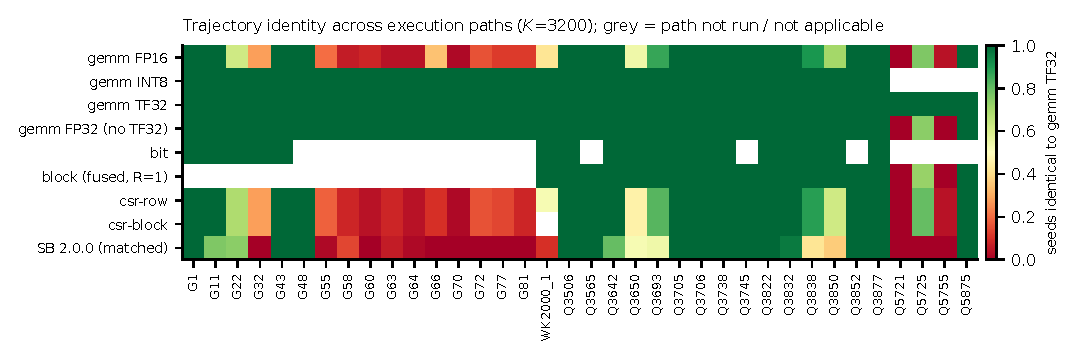
\includegraphics[width=\linewidth]{figS_trajectory_identity.pdf}
\caption{Trajectory identity across execution paths at $K=3200$: for every instance, the fraction of the 50 seeds whose final cut equals that of the \code{gemm} TF32 reference. Ternary instances (K2000, all G-set instances, QPLIB instances with couplings in $\{-1,0,+1\}$) give bitwise identical results for TF32, FP32, INT8, \code{bit} and \code{block}; the FP16-operand path and the CSR paths differ; on the four weighted QPLIB instances (5721, 5725, 5755, 5875) every reduced-precision path differs. Blank cells: path not run (\code{bit} does not fit for $n\ge3000$ at $B=512$; \code{block} was run on K2000 and QPLIB only).}
\label{fig:identity}
\end{figure}

\subsection{K2000}\label{sec:res-k2000}
On K2000 at $B=512$ the fastest path, \code{gemm} FP16, needs 12.4~\textmu s per integration step; \code{gemm} INT8 needs 16.0, \code{gemm} TF32 26.7, \code{bit} 30.1 and \code{gemm} FP32 without tensor cores 112, and the matched public package 170~\textmu s (Figure~\ref{fig:k2000}, Table~\ref{tab:k2000}). Every path is linear in $K$ to within 3\% over the sixteen-fold range of the step grid (Table~\ref{tab:steps}), so the per-step time is a property of the path and the instance alone. On the integration boundary the fastest path is therefore $13.6\times$ faster than the package at equal work, whereas the tensor-core-free FP32 product is only $1.5\times$ faster: on this instance most of the speedup is arithmetic throughput rather than dispatch overhead.

\begin{figure}[!ht]\centering
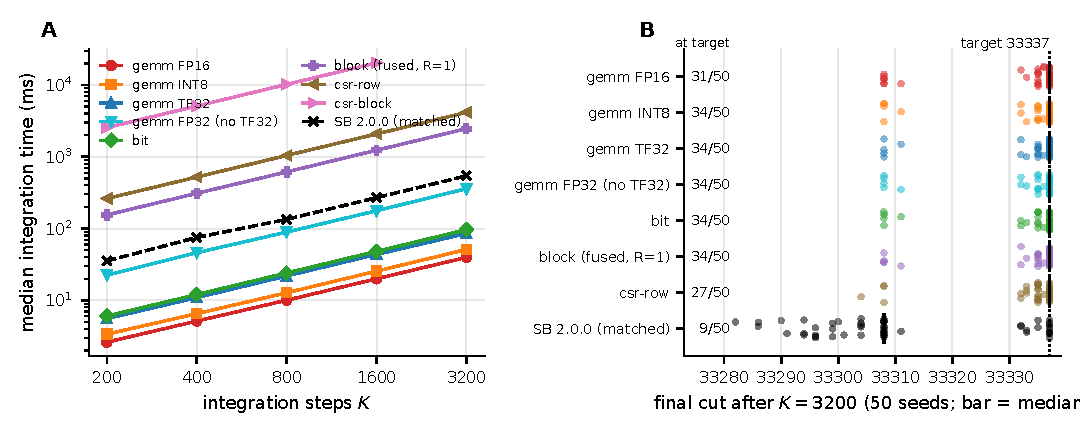
\includegraphics[width=\linewidth]{fig1_k2000_dense.pdf}
\caption{K2000 ($n=2000$, complete graph, $B=512$, $\Delta t=1.10$, 50 independent trials per configuration; SB~2.0.0 with the matched schedule). Panel~A: median integration time against the step budget for the main execution paths. Panel~B: distribution of the final cut at $K=3200$ (one dot per trial, bar = median; left column = trials reaching the target 33337). The FP32-state dense paths return identical cuts in all 50 trials.}
\label{fig:k2000}
\end{figure}

\begin{table}[!ht]\centering\small
\caption{K2000 at $B=512$, $K=3200$, target 33337, 50 independent trials per configuration. Solve time is the median integration time. $u/M$ counts trials whose best replica reached the target; TTS$_{99}$ follows Eq.~\eqref{eq:restarts} on the integration boundary.}
\label{tab:k2000}
% auto-generated: K2000, B=512, K=3200, target 33337, matched SB 2.0.0 baseline
\begin{tabular}{lrrrrrr}\toprule
Path & \textmu s/step & Solve (ms) & Best & Median & $u/M$ & TTS$_{99}$ (s)\\\midrule
SB 2.0.0 (matched) & 169.5 & 542.4 & 33337 & 33308.0 & 9/50 & 13 \\
\texttt{csr-row} & 1298.6 & 4155.4 & 33337 & 33337.0 & 27/50 & 24.9 \\
\texttt{block} & 770.7 & 2466.3 & 33337 & 33337.0 & 34/50 & 12.3 \\
\texttt{gemm} FP32 (no TF32) & 112.4 & 359.8 & 33337 & 33337.0 & 34/50 & 1.8 \\
\texttt{gemm} TF32 & 26.7 & 85.5 & 33337 & 33337.0 & 34/50 & 0.428 \\
\texttt{gemm} INT8 & 16.0 & 51.2 & 33337 & 33337.0 & 34/50 & 0.256 \\
\texttt{bit} & 30.1 & 96.4 & 33337 & 33337.0 & 34/50 & 0.482 \\
\texttt{gemm} FP16 & 12.4 & 39.8 & 33337 & 33337.0 & 31/50 & 0.199 \\
\bottomrule\end{tabular}

\end{table}

\begin{table}[!ht]\centering\small
\caption{K2000 step-budget sweep at $B=512$, 50 trials per cell. Upper block: median integration time. Lower block: median cut and, in parentheses, trials reaching the target 33337. The FP32, TF32, INT8, \code{bit} and \code{block} paths share one objective row because their trajectories are identical.}
\label{tab:steps}
\resizebox{\linewidth}{!}{% auto-generated: K2000 step-budget sweep, B=512, 50 trials per cell
\begin{tabular}{lrrrrr}\toprule
 & $K=200$ & $K=400$ & $K=800$ & $K=1600$ & $K=3200$\\\midrule
\multicolumn{6}{l}{\emph{Median integration time} (ms)}\\
SB 2.0.0 (matched) & 35.51 & 75.29 & 134.55 & 269.86 & 542.43\\
\texttt{csr-row} & 261.93 & 522.25 & 1043.83 & 2079.19 & 4155.42\\
\texttt{block} & 154.96 & 309.79 & 615.41 & 1234.07 & 2466.32\\
\texttt{gemm} FP32 (no TF32) & 22.48 & 46.11 & 89.29 & 177.23 & 359.79\\
\texttt{gemm} TF32 & 5.58 & 10.94 & 21.92 & 43.72 & 85.51\\
\texttt{gemm} INT8 & 3.38 & 6.53 & 12.77 & 25.55 & 51.21\\
\texttt{bit} & 6.05 & 12.06 & 24.08 & 48.18 & 96.35\\
\texttt{gemm} FP16 & 2.62 & 5.15 & 10.05 & 19.99 & 39.78\\
\midrule
\multicolumn{6}{l}{\emph{Median objective} / trials reaching target}\\
SB 2.0.0 (matched) & 32916.5 (0) & 33131.0 (0) & 33243.5 (0) & 33278.5 (1) & 33308.0 (9)\\
\texttt{csr-row} & 33177.5 (0) & 33250.0 (0) & 33290.5 (1) & 33309.5 (10) & 33337.0 (27)\\
\texttt{block} & 33177.5 (0) & 33252.0 (0) & 33290.5 (1) & 33311.0 (11) & 33337.0 (34)\\
\texttt{gemm} FP32 (no TF32) & 33177.5 (0) & 33252.0 (0) & 33290.5 (1) & 33311.0 (11) & 33337.0 (34)\\
\texttt{gemm} TF32 & 33177.5 (0) & 33252.0 (0) & 33290.5 (1) & 33311.0 (11) & 33337.0 (34)\\
\texttt{gemm} INT8 & 33177.5 (0) & 33252.0 (0) & 33290.5 (1) & 33311.0 (11) & 33337.0 (34)\\
\texttt{bit} & 33177.5 (0) & 33252.0 (0) & 33290.5 (1) & 33311.0 (11) & 33337.0 (34)\\
\texttt{gemm} FP16 & 33178.5 (0) & 33250.0 (0) & 33291.0 (0) & 33309.5 (7) & 33337.0 (31)\\
\bottomrule\end{tabular}
}
\end{table}

The TTS on K2000 is 0.20~s for \code{gemm} FP16, 0.26~s for INT8, 0.43~s for TF32 and 0.48~s for \code{bit}, against 13~s for the package, all at $K=3200$ (Table~\ref{tab:k2000}). Two further features of the table are reported before any ratio is interpreted. First, the solution quality of the custom paths is higher than that of the matched package at every budget: at $K=3200$, 34 of 50 trials reach the target against 9 of 50, and the median cut is 33337 against 33308; at $K=200$ the medians are 33177.5 against 32916.5. Since the schedule is matched, this residual difference must come from the remaining rows of Table~\ref{tab:align}---the gain normalisation and the order of operations within a step---and we do not attribute it to the arithmetic. The success probability rises steeply with $K$ (1, 11 and 34 of 50 at $K=800$, 1600 and 3200, Figure~\ref{fig:sensitivity}C), so the time to solution is minimised at the largest budget measured. Second, the dense fused \code{block} path is $29\times$ slower than the library path on this instance, and \code{csr-row} is $49\times$ slower; the reason for the former is the occupancy argument of Section~\ref{sec:occupancy}, and the latter is the expected cost of a sparse representation on a complete graph. Figure~\ref{fig:panorama} places all fifteen execution paths, including the cluster and global-synchronisation variants, on one scale: the spread between the best and the worst path on the same instance is three orders of magnitude, which is the cost of choosing the storage format and synchronisation scheme wrongly.

\begin{figure}[!ht]\centering
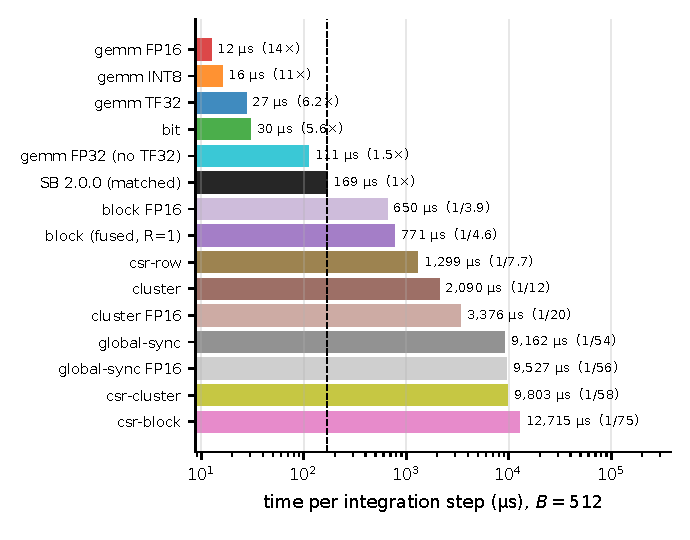
\includegraphics[width=0.62\linewidth]{figS_k2000_all_paths.pdf}
\caption{Time per integration step of all fifteen execution paths on K2000 at $B=512$, $K=1600$. The dashed line is SB~2.0.0 with the matched schedule; numbers in parentheses are speedups (or slowdowns) relative to it.}
\label{fig:panorama}
\end{figure}

\subsection{G-set}\label{sec:res-gset}
Table~\ref{tab:gset} and Figure~\ref{fig:instances} report, for each of the 16 G-set instances at $K=3200$, the path with the smallest integration time and its comparison with the matched package. The fastest path is \code{csr-block} on the eight instances with average degree at most four (the toroidal and planar families G11, G32, G48, G66, G70, G72, G77, G81), \code{csr-row} on the two degree-five instances (G55, G60), \code{gemm} FP16 on four of the six instances with average degree between 12 and 48 (G1, G22, G43, G58), and the exact \code{gemm} INT8 path on the remaining two (G63, G64, $n=7000$), where it is 7\% faster than FP16. The integration speedup ranges from $13.5\times$ (G22) to $137\times$ (G81) with a median of $27\times$. The package's per-step time is flat at about 170~\textmu s up to $n=2000$ and then grows as $n^2$ (290~\textmu s at $n=3000$, 1078 at 7000, 8761 at 20,000), because it stores the coupling matrix densely; the CSR paths grow with the nonzero count instead, which is why the speedup increases with $n$ on the sparse families.

\begin{table}[!ht]\centering\footnotesize\setlength{\tabcolsep}{3.5pt}
\caption{G-set at $K=3200$, $B=512$: fastest custom path by integration time, compared with SB~2.0.0 under the matched schedule. ``deg'' is the average degree $2|\mathcal E|/n$; gaps are median gaps to the best-known cut over 50 trials; $u$ counts trials reaching the best-known cut.}
\label{tab:gset}
\resizebox{\linewidth}{!}{% auto-generated: G-set, K=3200, fastest dsb-gpu path (integration time) vs matched SB 2.0.0
\begin{tabular}{lrrrrlrrrrrr}\toprule
Instance & $n$ & deg & $B$ & $\Delta t$ & Fastest path & \textmu s/step & SB \textmu s/step & Speedup & Gap (\%) & SB gap (\%) & $u$ dsb/SB\\\midrule
G1 & 800 & 47.9 & 512 & 0.58 & \texttt{gemm} FP16 & 6.4 & 174.9 & 27.3 & 0.000 & 0.000 & 50/50 \\
G11 & 800 & 4.0 & 512 & 1.18 & \texttt{csr-block} & 3.1 & 173.5 & 56.0 & 0.000 & 0.000 & 50/38 \\
G43 & 1000 & 20.0 & 512 & 0.71 & \texttt{gemm} FP16 & 7.3 & 191.8 & 26.3 & 0.000 & 0.000 & 50/50 \\
G22 & 2000 & 20.0 & 512 & 0.71 & \texttt{gemm} FP16 & 12.3 & 166.1 & 13.5 & 0.007 & 0.007 & 13/5 \\
G32 & 2000 & 4.0 & 512 & 1.17 & \texttt{csr-block} & 6.9 & 166.3 & 24.0 & 0.284 & 0.993 & 0/0 \\
G48 & 3000 & 4.0 & 512 & 1.10 & \texttt{csr-block} & 9.6 & 290.0 & 30.1 & 0.000 & 0.000 & 50/50 \\
G55 & 5000 & 5.0 & 512 & 0.93 & \texttt{csr-row} & 29.1 & 662.3 & 22.7 & 0.175 & 0.243 & 0/0 \\
G58 & 5000 & 11.8 & 512 & 0.51 & \texttt{gemm} FP16 & 42.6 & 662.9 & 15.6 & 0.376 & 0.394 & 0/0 \\
G60 & 7000 & 4.9 & 512 & 0.93 & \texttt{csr-row} & 40.7 & 1076.4 & 26.4 & 0.204 & 0.275 & 0/0 \\
G63 & 7000 & 11.8 & 512 & 0.50 & \texttt{gemm} INT8 & 70.2 & 1079.4 & 15.4 & 0.399 & 0.410 & 0/0 \\
G64 & 7000 & 11.8 & 512 & 0.58 & \texttt{gemm} INT8 & 70.6 & 1078.2 & 15.3 & 0.891 & 0.777 & 0/0 \\
G66 & 9000 & 4.0 & 512 & 1.16 & \texttt{csr-block} & 27.5 & 1808.2 & 65.8 & 1.069 & 1.760 & 0/0 \\
G70 & 10000 & 2.0 & 512 & 0.98 & \texttt{csr-block} & 30.8 & 2274.3 & 73.8 & 1.324 & 1.762 & 0/0 \\
G72 & 10000 & 4.0 & 512 & 1.16 & \texttt{csr-block} & 31.1 & 2273.6 & 73.0 & 1.056 & 1.769 & 0/0 \\
G77 & 14000 & 4.0 & 512 & 1.15 & \texttt{csr-block} & 46.2 & 4326.8 & 93.7 & 1.006 & 1.751 & 0/0 \\
G81 & 20000 & 4.0 & 512 & 1.15 & \texttt{csr-block} & 64.1 & 8761.5 & 136.7 & 1.110 & 1.821 & 0/0 \\
\bottomrule\end{tabular}
}
\end{table}

\begin{figure}[!ht]\centering
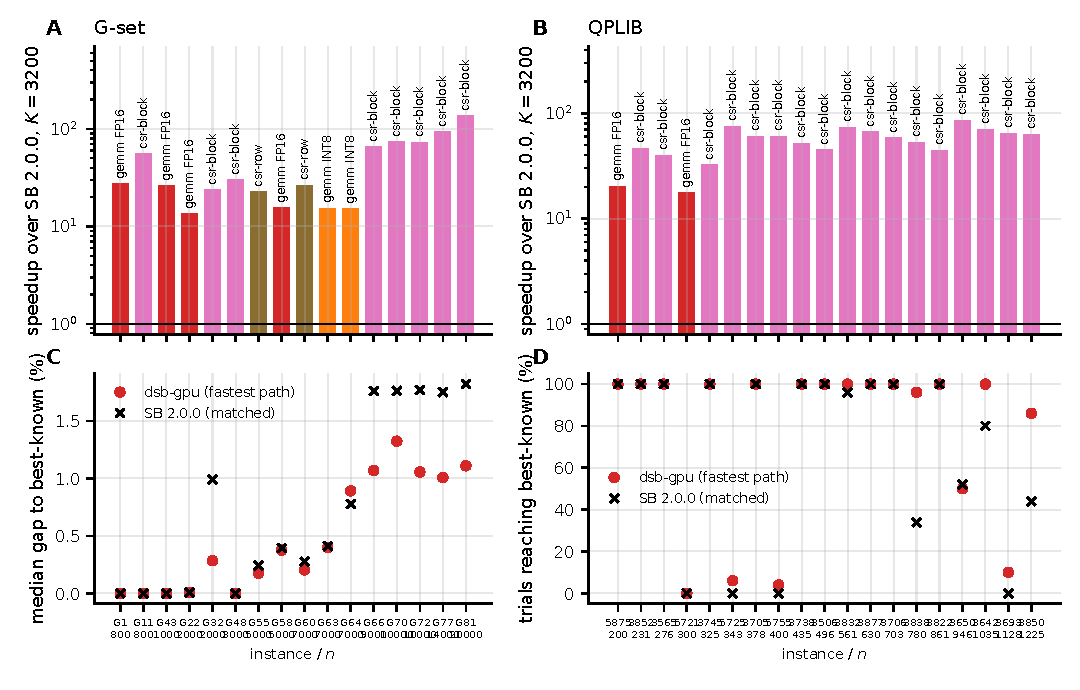
\includegraphics[width=\linewidth]{fig6_gset_qplib.pdf}
\caption{Per-instance comparison at $K=3200$ against SB~2.0.0 with the matched schedule. Panels~A, B: speedup of the fastest custom path (selected by integration time; path named above each bar) for 16 G-set instances ($B=512$) and 19 QPLIB instances ($B=256$--$2048$). Panel~C: median gap to the best-known cut over 50 trials on G-set. Panel~D: fraction of the 50 trials reaching the best-known value on QPLIB.}
\label{fig:instances}
\end{figure}

Solution quality at equal work is at least as good as the package's on 15 of the 16 instances: the median gap is lower on ten (most clearly on the sparse large instances, where the package's gap is 1.75--1.82\% against 1.0--1.3\%, and on G32, 0.28\% against 0.99\%), equal on five, and higher on one (G64, 0.89\% against 0.78\%). The instances on which the best-known cut is reached at all lie at $n\le3000$. On G1, G11, G43 and G48 the custom TTS$_{99}$ at $K=3200$ is 10--31~ms against 0.55--2.2~s for the package (G1: 0.020~s against 0.56~s; G11: 0.010~s against 2.2~s; G48: 0.031~s against 0.93~s); on G22 it is 0.63~s against 23~s; on G32 a single FP16 trial reached the best-known cut and the estimate is not interpreted. On the four small instances every trial already succeeds at a smaller budget, so the TTS over the step grid is lower still (G1: 10.3~ms at $K=1600$; G11: 5.0~ms at $K=1600$; G43: 11.8~ms at $K=1600$; G48: 2.0~ms at $K=200$); the literature comparison of Section~\ref{sec:res-literature} uses this per-instance choice of budget, which is the published practice. On the ten instances with $n\ge5000$ neither implementation reaches the best-known cut in any of the 50 trials at $K=3200$, so the comparison there rests on the gap alone and TTS$_{99}$ is unresolved for both.

\subsection{QPLIB}\label{sec:res-qplib}
Table~\ref{tab:qplib} reports the 19 QPLIB instances. The fastest path is \code{csr-block} on 17 of them and \code{gemm} FP16 on the two dense weighted instances 5721 and 5875. The integration speedup over the matched package ranges from $17.6\times$ to $86\times$ with a median of $58\times$. These are the largest ratios in the study and also the ones that must be read most carefully: the package needs 162--182~\textmu s per step on every QPLIB instance regardless of $n$ (200 to 1225) and $B$ (256 to 2048), exactly the floor observed on K2000 and the small G-set instances. At these sizes the package is bound by per-step host dispatch and not by arithmetic, so the QPLIB speedup measures the removal of that overhead by persistent kernels and graph capture, not tensor-core throughput. The custom paths at 2--4~\textmu s per step are themselves close to their own floor: one grid-wide or block-wide synchronisation per step.

Solution quality is at least as good as the package's on 17 of 19 instances. Both reach the reference value in every trial on ten instances; the custom path reaches it more often on 3838 (48 against 17 trials), 3850 (43 against 22), 3642 (50 against 40) and 3832 (50 against 48), and is the only one to reach it on 3693, 5725 and 5755. The package is marginally ahead on 3650 (26 against 25 trials) and, by median objective though not by success count, on 5725. Neither reaches the reference value of 5721. Where both succeed, TTS$_{99}$ is 8--50~ms against 0.5--6.6~s.

\begin{table}[!ht]\centering\footnotesize\setlength{\tabcolsep}{3.5pt}
\caption{QPLIB at $K=3200$: fastest custom path by integration time, compared with SB~2.0.0 under the matched schedule. $B$ is chosen by $n$; gaps are median gaps to the reference value over 50 trials; $u$ counts trials reaching it.}
\label{tab:qplib}
\resizebox{\linewidth}{!}{% auto-generated: QPLIB, K=3200, fastest dsb-gpu path (integration time) vs matched SB 2.0.0
\begin{tabular}{lrrrlrrrrrr}\toprule
Instance & $n$ & $B$ & $\Delta t$ & Fastest path & \textmu s/step & SB \textmu s/step & Speedup & Gap (\%) & SB gap (\%) & $u$ dsb/SB\\\midrule
QPLIB\_5875 & 200 & 1024 & 0.53 & \texttt{gemm} FP16 & 8.7 & 177.6 & 20.3 & 0.000 & 0.000 & 50/50 \\
QPLIB\_3852 & 231 & 2048 & 1.15 & \texttt{csr-block} & 3.7 & 173.3 & 46.4 & 0.000 & 0.000 & 50/50 \\
QPLIB\_3565 & 276 & 2048 & 1.17 & \texttt{csr-block} & 4.3 & 171.5 & 39.6 & 0.000 & 0.000 & 50/50 \\
QPLIB\_5721 & 300 & 512 & 1.03 & \texttt{gemm} FP16 & 10.0 & 174.9 & 17.6 & 0.786 & 0.821 & 0/0 \\
QPLIB\_3745 & 325 & 2048 & 1.17 & \texttt{csr-block} & 5.1 & 163.6 & 32.3 & 0.000 & 0.000 & 50/50 \\
QPLIB\_5725 & 343 & 1024 & 1.07 & \texttt{csr-block} & 2.3 & 174.0 & 74.7 & 0.099 & 0.000 & 3/0 \\
QPLIB\_3705 & 378 & 1024 & 1.15 & \texttt{csr-block} & 2.9 & 172.9 & 60.1 & 0.000 & 0.000 & 50/50 \\
QPLIB\_5755 & 400 & 1024 & 1.05 & \texttt{csr-block} & 2.9 & 175.0 & 60.6 & 0.425 & 0.661 & 2/0 \\
QPLIB\_3738 & 435 & 1024 & 1.16 & \texttt{csr-block} & 3.4 & 174.2 & 51.6 & 0.000 & 0.000 & 50/50 \\
QPLIB\_3506 & 496 & 1024 & 1.16 & \texttt{csr-block} & 4.0 & 181.7 & 44.9 & 0.000 & 0.000 & 50/50 \\
QPLIB\_3832 & 561 & 512 & 1.16 & \texttt{csr-block} & 2.4 & 172.8 & 73.0 & 0.000 & 0.000 & 50/48 \\
QPLIB\_3877 & 630 & 512 & 1.15 & \texttt{csr-block} & 2.6 & 175.9 & 66.6 & 0.000 & 0.000 & 50/50 \\
QPLIB\_3706 & 703 & 512 & 1.16 & \texttt{csr-block} & 3.0 & 172.7 & 58.4 & 0.000 & 0.000 & 50/50 \\
QPLIB\_3838 & 780 & 512 & 1.17 & \texttt{csr-block} & 3.2 & 171.8 & 52.9 & 0.000 & 0.268 & 48/17 \\
QPLIB\_3822 & 861 & 512 & 1.15 & \texttt{csr-block} & 3.7 & 162.1 & 44.3 & 0.000 & 0.000 & 50/50 \\
QPLIB\_3650 & 946 & 256 & 1.16 & \texttt{csr-block} & 2.0 & 174.3 & 85.6 & 0.108 & 0.000 & 25/26 \\
QPLIB\_3642 & 1035 & 256 & 1.16 & \texttt{csr-block} & 2.3 & 164.0 & 69.8 & 0.000 & 0.000 & 50/40 \\
QPLIB\_3693 & 1128 & 256 & 1.15 & \texttt{csr-block} & 2.5 & 164.3 & 64.6 & 0.173 & 0.173 & 5/0 \\
QPLIB\_3850 & 1225 & 256 & 1.16 & \texttt{csr-block} & 2.7 & 168.2 & 62.9 & 0.000 & 0.167 & 43/22 \\
\bottomrule\end{tabular}
}
\end{table}

\subsection{Comparison with the package's library defaults}\label{sec:res-library}
The matched schedule of Section~\ref{sec:align} changes the package's time step, pump and initial state. To show what the comparison looks like without that intervention, Figure~\ref{fig:library} runs the package with its library defaults on 66 G-set instances at $K=800$ against a single custom path, \code{csr-row}, with the per-instance time step. The integration speedup is $4.7$--$77\times$ (median $10.8\times$); the median gap is lower for \code{csr-row} on 64 of the 66 instances, the library configuration reaches the best-known cut on 3 instances against 30, and its gap grows with $n$ because the pump $\min(k/1000,1)$ reaches only $0.8$ within 800 steps. The comparison against library defaults is therefore more favourable to our implementation than the matched comparison on every axis; we report the matched numbers as the primary result precisely because the library-default numbers measure the schedule as much as the implementation.

\begin{figure}[!ht]\centering
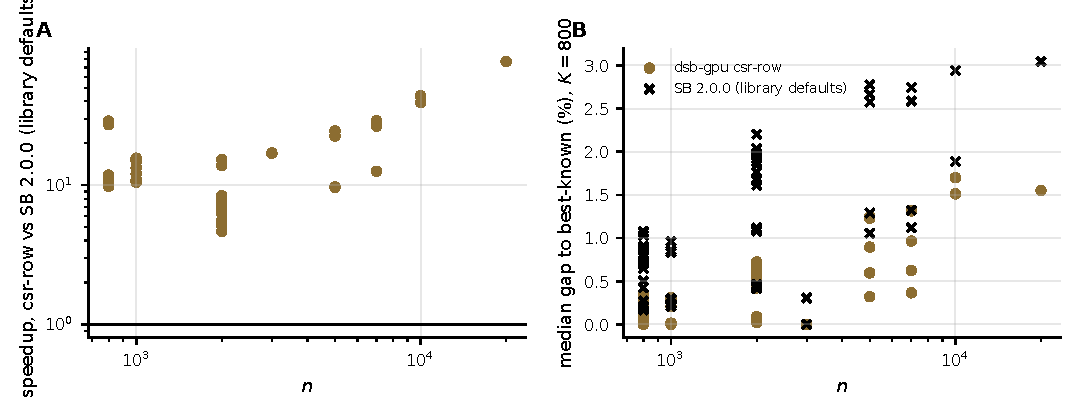
\includegraphics[width=\linewidth]{fig7_gset66_library_baseline.pdf}
\caption{66 G-set instances (G1--G63, G70, G72, G81) at $K=800$, $B=512$: \code{csr-row} against SB~2.0.0 with its library defaults (time step 0.1, pump $\min(k/1000,1)$, uniform$(-1,1)$ initial state). Panel~A: integration speedup. Panel~B: median gap to the best-known cut over 50 trials.}
\label{fig:library}
\end{figure}

\subsection{Comparison with published simulated-bifurcation machines}\label{sec:res-literature}
Table~\ref{tab:literature} compares the present implementation with published SB machines on the instances that they share with our benchmark set: the single-FPGA discrete SB machine (dSBM) and the single-GPU dSB of Goto et al.~\cite{goto2021}, and the CUDA dSB baseline of Tao et al.~\cite{tabu2026}. Table~\ref{tab:throughput} adds the coupling-product throughput on K2000 of the aSB machines of Tatsumura et al.~\cite{fpga2019}, which is the figure of merit that work reports. The published values are cited from the respective papers and their supplementary tables; we could not run those machines ourselves, so the comparison is limited to the instances and metrics reported there, and it crosses hardware generations (Arria~10 and Stratix~10 FPGAs, a Tesla V100, an RTX~4090 and the GH200) as well as SB variants. Goto et al.\ and Tao et al.\ define TTS as we do, $\mathrm{TTS}=T_{\mathrm{com}}\log(0.01)/\log(1-P_S)$ with $T_{\mathrm{com}}$ the computation time per batch and $P_S$ the success probability for the best-known cut (Section~\ref{sec:quality}), so the values are commensurable up to the choice of operating point. Goto et al.\ select $N_{\mathrm{step}}$ and $\Delta t$ per instance to minimise TTS and use $N_{\mathrm{batch}}=\lfloor 2048/n\rfloor$ on the FPGA and 80--160 on the GPU; Tao et al.\ fix 10,000 iterations and 1000 runs; for the present work we quote, for each instance, the fastest path and the best of the five step budgets at $B=512$ with the per-instance $\Delta t$ of Section~\ref{sec:step}.

\begin{table}[!ht]\centering\footnotesize\setlength{\tabcolsep}{4pt}
\caption{Time to solution of the present implementation and of published dSB machines on the shared instances. Every row uses $\mathrm{TTS}=T_{\mathrm{com}}\log(0.01)/\log(1-P_S)$ with the best-known cut as target; $T_{\mathrm{com}}$ is the computation time per batch of $N_{\mathrm{batch}}$ trials (integration boundary here; excluding data loading in \cite{goto2021}). Published values are cited from the tables indicated. ``$>$'' marks a lower bound where the target was not reached in any run ($P_S<10^{-3}$); ``---'' marks a quantity the work does not report. Present work: GH200, 50 independent trials, integration boundary, fastest path and best step budget per instance.}
\label{tab:literature}
\resizebox{\linewidth}{!}{%
\begin{tabular}{llllrrrr}\toprule
Instance ($n$, target) & Work & Hardware & Algorithm & $N_{\mathrm{step}}$ & $\Delta t$ & $N_{\mathrm{batch}}$ & TTS \\
\midrule
K2000 (2000, 33337) & Goto et al.\ 2021 \cite{goto2021}, Table~S1 & Stratix~10 GX FPGA & dSBM, 1-bit $J$   & 9000   & 1.25 & 1   & 1.34~s \\
                    & Goto et al.\ 2021 \cite{goto2021}, Table~S3 & Tesla V100         & dSB               & 40{,}000 & 0.25 & 80  & 1.70~s \\
                    & Tao et al.\ 2026 \cite{tabu2026}, Table~1   & RTX 4090           & dSB (CUDA)        & 10{,}000 & ---  & --- & $4.3\times10^{3}$~s \\
                    & Present work                                & GH200              & dSB, \code{gemm} FP16        & 3200 & 1.10 & 512 & \textbf{0.20~s} \\
                    & Present work                                & GH200              & dSB, \code{gemm} INT8 (exact) & 3200 & 1.10 & 512 & 0.26~s \\
\midrule
G1 (800, 11624)     & Goto et al.\ 2021 \cite{goto2021}, Table~S2 & Stratix~10 GX FPGA & dSBM, 2-bit $J$   & 9000   & 0.5  & 2   & 32.2~ms \\
                    & Goto et al.\ 2021 \cite{goto2021}, Table~S3 & Tesla V100         & dSB               & 2000   & 0.5  & 160 & 33.3~ms \\
                    & Tao et al.\ 2026 \cite{tabu2026}, Table~1   & RTX 4090           & dSB (CUDA)        & 10{,}000 & ---  & --- & 443~s \\
                    & Present work                                & GH200              & dSB, \code{gemm} FP16 & 1600 & 0.58 & 512 & \textbf{10.3~ms} \\
\midrule
G11 (800, 564)      & Goto et al.\ 2021 \cite{goto2021}, Table~S2 & Stratix~10 GX FPGA & dSBM, 2-bit $J$   & 5000   & 1.25 & 2   & 19.9~ms \\
                    & Present work                                & GH200              & dSB, \code{csr-block} & 1600 & 1.18 & 512 & \textbf{5.0~ms} \\
\midrule
G22 (2000, 13359)   & Goto et al.\ 2021 \cite{goto2021}, Table~S1 & Stratix~10 GX FPGA & dSBM, 2-bit $J$   & 30{,}000 & 0.75 & 1   & 2.67~s \\
                    & Tao et al.\ 2026 \cite{tabu2026}, Table~1   & RTX 4090           & dSB (CUDA)        & 10{,}000 & ---  & --- & $>6.7\times10^{3}$~s \\
                    & Present work                                & GH200              & dSB, \code{gemm} FP16 & 3200 & 0.71 & 512 & \textbf{0.63~s} \\
\bottomrule
\end{tabular}}
\end{table}

\begin{table}[!ht]\centering\footnotesize\setlength{\tabcolsep}{5pt}
\caption{Coupling-product throughput on K2000 ($n=2000$). $T_{\mathrm{step}}$ is the time of one integration step for the number of trials processed in parallel; throughput is $n^{2}N_{\mathrm{batch}}/T_{\mathrm{step}}$ in giga multiply--accumulates per second, the figure of merit of \cite{fpga2019} (its Table~II). Present work: median over 50 trials at $K=3200$.}
\label{tab:throughput}
\begin{tabular}{lllrrr}\toprule
Work & Hardware & Algorithm & Trials per step & $T_{\mathrm{step}}$ (\textmu s) & GMAC/s \\
\midrule
Tatsumura et al.\ 2019 \cite{fpga2019} & Arria~10 GX~1150 FPGA & aSB, 2K design & 1   & 2.2  & 1{,}873 \\
Tatsumura et al.\ 2019 \cite{fpga2019} & Tesla V100            & aSB            & 1   & 36   & 113 \\
Present work & GH200 & dSB, \code{gemm} FP16 & 512 & 12.4 & $1.65\times10^{5}$ \\
Present work & GH200 & dSB, \code{gemm} INT8 (exact) & 512 & 16.0 & $1.28\times10^{5}$ \\
Present work & GH200 & dSB, \code{gemm} TF32 (exact) & 512 & 26.7 & $0.77\times10^{5}$ \\
Present work & GH200 & dSB, \code{bit} (exact)       & 512 & 30.1 & $0.68\times10^{5}$ \\
Present work & GH200 & dSB, \code{bit} (exact)       & 16  & 3.2  & $0.20\times10^{5}$ \\
\bottomrule
\end{tabular}
\end{table}

On K2000 the TTS of the present implementation is 0.20~s with FP16 operands and 0.26~s with the exact INT8 path, against 1.34~s for the dSBM, 1.70~s for the V100 dSB and $4.3\times10^{3}$~s for the CUDA dSB baseline of Tao et al. On G1 it is 10.3~ms against 32.2~ms (dSBM) and 33.3~ms (V100); on G11, 5.0~ms against 19.9~ms; on G22, 0.63~s against 2.67~s for the dSBM, while the CUDA baseline of Tao et al.\ did not reach the best-known cut in 1000 runs. In throughput terms (Table~\ref{tab:throughput}), one 512-replica step of the FP16 path on K2000 delivers $1.65\times10^{5}$~GMAC/s of coupling products, $88\times$ the 1,873~GMAC/s of the 2048-spin FPGA design of \cite{fpga2019} and $1.5\times10^{3}$ times the single-trial V100 implementation reported in the same work, which reads the coupling matrix from HBM2 at every step and is bandwidth-bound. The dSBM of \cite{goto2021}, which stores K2000 with one bit per coupling, needs about 0.29~\textmu s per step for a single trial (inferred from its Table~S1 as $T_{\mathrm{com}}=\mathrm{TTS}\log(1-P_S)/\log 0.01$ divided by $N_{\mathrm{step}}$), i.e.\ $1.4\times10^{4}$~GMAC/s, a factor of 12 below the FP16 path and a factor of 9 below the exact INT8 path. Even with 16 replicas, the fused \code{bit} kernel delivers $2.0\times10^{4}$~GMAC/s at 3.2~\textmu s per step (Section~\ref{sec:res-sensitivity}). At $B=128$, the batch size closest to the 80--160 trials of the V100 dSB of Goto et al., the TTS on K2000 at $K=3200$ is 0.50~s with FP16 operands and 0.78~s with the exact \code{bit} or INT8 paths, still below the 1.70~s reported for that implementation.

Two qualifications apply. First, the published operating points were chosen per instance to minimise TTS, with $N_{\mathrm{step}}$ up to 40,000 on the GPU and 30,000 on the FPGA, whereas the largest budget measured here is 3200. On the instances where the success probability is still rising at $K=3200$ (K2000 and G22, Section~\ref{sec:res-sensitivity}) a larger budget would lower our TTS further, so the present-work entries of Table~\ref{tab:literature} are upper bounds in that sense. Second, the FPGA machines process one or two trials with a per-step latency of 0.3--2.5~\textmu s, well below the 12.4~\textmu s of a 512-replica step here; the shortest step measured in this work, 3.2~\textmu s for 16 replicas with the fused \code{bit} kernel, is within a factor of 1.5 of the 2048-spin aSB FPGA but an order of magnitude above the dSBM. The GPU advantage is throughput, obtained by amortising each read of the coupling matrix over many replicas; it does not carry over to latency-bound settings such as the real-time control loops for which the FPGA machines were designed \cite{tatsumura2021heart}, and on instances that are solved within a few hundred steps the difference in per-step latency matters more than the difference in throughput.

\subsection{Arithmetic modes and the measured path-selection region}\label{sec:res-region}
Table~\ref{tab:arith} compares the arithmetic modes on the same instance against the \code{gemm} TF32 reference, as a median over instances of each family, together with the identity fraction of Figure~\ref{fig:identity}. Within the exact group the ratios are pure execution effects. INT8 is $1.67$--$2.31\times$ faster than TF32 on every family and, on all eight G-set instances with $n\ge7000$, as fast as or faster than FP16 operands (70 against 75~\textmu s per step on G60--G64, 98 against 116 on G66, 238 against 259 on G77 and 362 against 498 on G81, equal on G70 and G72), so that at these sizes the exact path is also the fastest dense one; FP16 operands are $2.2\times$ faster on K2000 and G-set, where the product dominates, and no faster on QPLIB, where the step is dispatch-bound. Disabling the tensor cores costs $4$--$5\times$ on K2000 and G-set but only $1.3\times$ on QPLIB, which is a second way of seeing that the QPLIB speedup is not arithmetic. The \code{bit} path is slower than TF32 on K2000 and G-set at $B=512$ ($0.89\times$ and $0.57\times$): its per-step time grows almost linearly with $B$, so at this batch size the population-count pipeline completes fewer $\pm1$ multiply-accumulates per cycle than the tensor cores. The ordering reverses at small batches, where the fused kernel's absence of per-step launches dominates and \code{bit} becomes the fastest path of all (Section~\ref{sec:res-sensitivity}). The dense fused \code{block} path is $0.03\times$ on K2000 and $0.19\times$ on QPLIB, for the occupancy reason of Section~\ref{sec:occupancy}.

\begin{table}[!ht]\centering\small
\caption{Arithmetic-mode comparison at $K=3200$. Ratio $=t(\text{\code{gemm} TF32})/t(\text{path})$ on the same instance, median over the instances of each family (number of instances in parentheses); ``identical'' is the mean over instances of the fraction of seeds whose final cut equals the TF32 reference.}
\label{tab:arith}
% auto-generated: ratio = t(gemm TF32)/t(path) on the same instance, median over instances (count); identity = mean fraction of seeds with final cut identical to gemm TF32
\begin{tabular}{lcccc}\toprule
Path & Identical to TF32 & K2000 & G-set & QPLIB\\\midrule
\texttt{gemm} TF32 & 1.00 & 1.00 (1) & 1.00 (16) & 1.00 (19)\\
\texttt{gemm} FP32 (no TF32) & 0.94 & 0.24 (1) & 0.19 (16) & 0.75 (19)\\
\texttt{gemm} INT8 & 1.00 & 1.67 (1) & 2.31 (16) & 1.87 (15)\\
\texttt{gemm} FP16 & 0.62 & 2.15 (1) & 2.19 (16) & 1.00 (19)\\
\texttt{bit} & 1.00 & 0.89 (1) & 0.57 (5) & 1.01 (12)\\
\texttt{block} & 0.89 & 0.03 (1) & --- & 0.19 (19)\\
\texttt{csr-row} & 0.61 & 0.02 (1) & 3.05 (16) & 2.27 (19)\\
\texttt{csr-block} & 0.61 & --- & 3.68 (16) & 4.80 (19)\\
\bottomrule\end{tabular}

\end{table}

Figure~\ref{fig:region} turns the per-instance results into a selection map. Panel~A plots the per-step time of the dense paths against $n$ at $B=512$: they depend on $n$ only, not on the graph, whereas the CSR paths depend on the nonzero count and appear as a scatter below the dense curves wherever the graph is sparse. Panel~B marks, for each G-set and K2000 instance, the fastest path in the plane of $n$ and average degree. The boundary is a boundary in degree, not in $n$: \code{csr-block} wins for degree at most four at every $n$ from 800 to 20,000, \code{csr-row} for degree five, and \code{gemm} FP16 for degree twelve and above, up to and including the complete graph. The mechanism is the one of Section~\ref{sec:model}: \code{csr-block} re-reads the CSR arrays once per replica per step, which is cheap only when they are small enough to live in L2, and \code{csr-row} pays one grid-wide barrier per step; the dense product is indifferent to sparsity and wins once the nonzero count per row approaches the point where its tensor-core throughput beats the irregular sparse accesses.

\begin{figure}[!ht]\centering
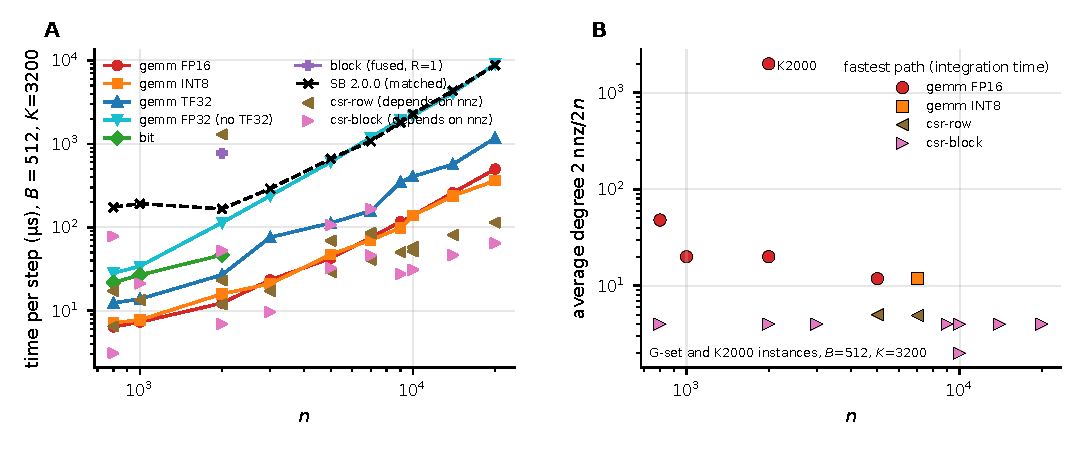
\includegraphics[width=\linewidth]{fig5_path_selection.pdf}
\caption{Measured path-selection region at $K=3200$, $B=512$. Panel~A: time per step against $n$ for the dense paths and SB~2.0.0 on the G-set and K2000 instances; the dense paths depend on $n$ only, whereas the CSR paths (scatter) depend on the nonzero count. SB~2.0.0 has a dispatch-bound floor of about 170~\textmu s per step for $n\le 2000$. Panel~B: fastest path by integration time for every G-set and K2000 instance in the plane of $n$ and average degree: \code{csr-block} up to degree four, \code{csr-row} at degree five, \code{gemm} FP16 or INT8 from degree twelve upward.}
\label{fig:region}
\end{figure}

The measurements therefore support a simple selection rule at $B=512$: \code{csr-block} for average degree below five, \code{csr-row} between five and about eight, \code{gemm} FP16 above for $n$ up to about 5000 and \code{gemm} INT8, which is exact and at least as fast, for larger dense instances. The rule depends on $B$ as well as on the instance: on K2000 with $B\le64$ the fused \code{bit} kernel is the fastest path (Section~\ref{sec:res-sensitivity}), and it is also the only dense format with a storage cost below one byte per coupling.

\subsection{Sensitivity to batch size and step budget}\label{sec:res-sensitivity}
Figure~\ref{fig:sensitivity} varies the number of replicas on the six largest G-set instances ($n=5000$--$20{,}000$) from $B=512$ to $8192$ at $K=3200$. The per-step time of the persistent CSR kernel is linear in $B$ over the whole range (Panel~A), so the kernel is compute- or bandwidth-bound rather than dispatch-bound already at $B=512$, and larger batches buy proportionally more replicas at constant throughput. They buy little in quality: the median gap to the best-known cut falls by 0.03--0.09 percentage points between $B=512$ and $B=8192$ (Panel~B), and the best of 50 trials does not reach the best-known value on any of the six instances at any batch size. For these instances the limiting factor is the dynamics, not the sampling budget, and the time to solution remains unresolved. Panel~C shows the complementary dependence on $K$ on K2000: the fraction of trials reaching the target rises from 2\% at $K=800$ to 22\% at 1600 and 68\% at 3200 for the exact paths, against 2\% and 18\% for the package at 1600 and 3200, so the optimal budget for time to solution lies at or beyond the largest step count measured.

\begin{figure}[!ht]\centering
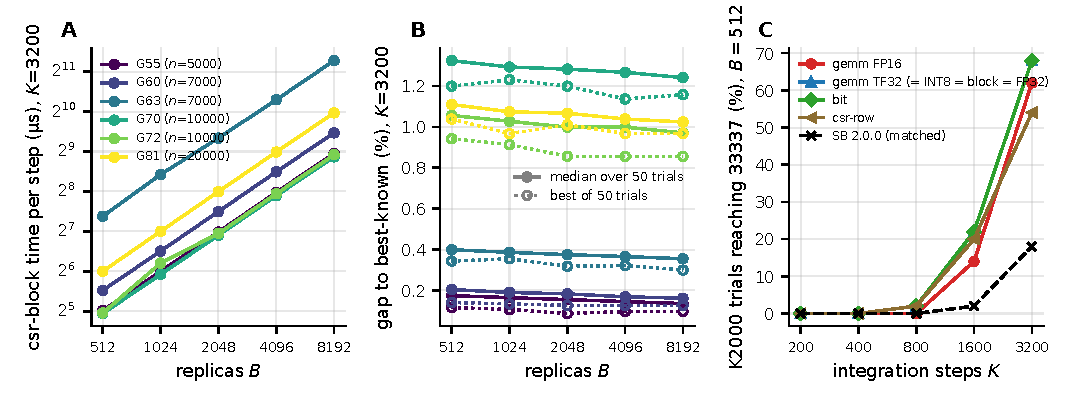
\includegraphics[width=\linewidth]{fig4_sensitivity.pdf}
\caption{Sensitivity to batch size and step budget. Panel~A: \code{csr-block} time per step against the number of replicas $B$ on the six largest G-set instances at $K=3200$. Panel~B: median (solid) and best (dotted) gap to the best-known cut over 50 trials against $B$ for \code{csr-block} on the same instances. Panel~C: K2000, fraction of trials reaching the target 33337 against $K$ at $B=512$.}
\label{fig:sensitivity}
\end{figure}

The replica count also decides which path is fastest. Figure~\ref{fig:k2000batch} repeats the K2000 benchmark at $B=16$, 64 and 128 for the exact \code{bit}, INT8 and TF32 paths, \code{gemm} FP16 and the matched package, with 50 trials and the same five step budgets. The graph-captured products have a floor: \code{gemm} FP16 needs 6.8--7.5~\textmu s per step and INT8 8.6--9.0~\textmu s at every $B$ up to 128, only $1.7$--$1.9\times$ less than at $B=512$, because every step still executes a library product and an update kernel. The fused \code{bit} kernel has no such floor. Its per-step time is 3.2~\textmu s at $B=16$, 5.7 at 64, 9.1 at 128 and 30.1 at 512, nearly proportional to $B$ above 64, so it is the fastest path at $B=16$ ($2.2\times$ faster than FP16 and $55\times$ faster than the package's 175~\textmu s) and at $B=64$ (5.7 against 6.8~\textmu s), and the crossover to the tensor-core products lies between 64 and 128 replicas. The package needs 168--175~\textmu s per step at every $B$, the dispatch floor of Section~\ref{sec:res-k2000}. The exact group remains bitwise identical at every batch size and step budget (at $K=3200$, 2, 4, 8 and 34 of 50 trials reach the target for $B=16$, 64, 128 and 512; FP16 3, 6, 10 and 31; the package 0, 2, 0 and 9). Because the probability that a batch contains the target grows faster with $B$ than the per-step time does, the time to solution at $K=3200$ decreases monotonically with $B$ for every path: for \code{gemm} FP16 it is 0.81~s at $B=64$, 0.50~s at $B=128$ and 0.20~s at $B=512$, and for the exact \code{bit} and INT8 paths 0.78~s at $B=128$ against 0.48 and 0.26~s at $B=512$; at $B=16$ at most three trials reach the target, so those estimates are not interpreted. The small-batch regime is therefore the one in which the fused bit-packed kernel is preferred, for per-step latency and for trials that must be short, whereas on this instance the time to solution favours the largest batch.

\begin{figure}[!ht]\centering
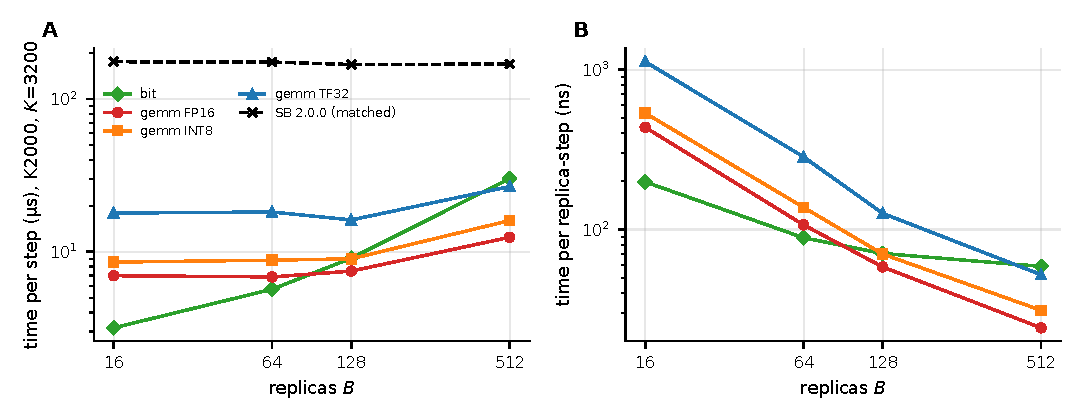
\includegraphics[width=\linewidth]{figS_k2000_batch.pdf}
\caption{K2000 batch sweep at $K=3200$ ($B\in\{16,64,128,512\}$, 50 trials per configuration, matched SB~2.0.0 schedule). Panel~A: time per integration step. Panel~B: time per replica-step (per-step time divided by $B$). The fused \code{bit} kernel is fastest for $B\le64$, the tensor-core products for $B\ge128$; the TF32, INT8 and \code{bit} trajectories are identical at every $B$.}
\label{fig:k2000batch}
\end{figure}

\subsection{Sparse scaling}\label{sec:res-sparse}
Figure~\ref{fig:sparse} reports the \code{csr-row} path on regular bipartite graphs of degree 100 with $n$ from 10,000 to 200,000 ($10^7$ nonzeros), $B=200$, at $K=200$ and $K=400$. The integration time is linear in $n$, in $K$ and in the nonzero count: every nonzero is updated in 0.152--0.156~ns per step across the twenty-fold range of $n$, a throughput of $0.65\times10^{12}$ nonzero updates per second, and the GPU allocation grows from 28~MB to 561~MB. The matched package, which stores the coupling matrix densely, takes $8.1\times$, $14.1\times$ and $33.2\times$ longer at $n=10^4$, $2\times10^4$ and $5\times10^4$, and could not be run at $n\ge10^5$, where its dense FP32 matrix would need 40~GB and then 160~GB. All trials of both implementations reach the planted optimum on every graph, as expected for this construction; these instances establish throughput and capacity, not optimization quality.

\begin{figure}[!ht]\centering
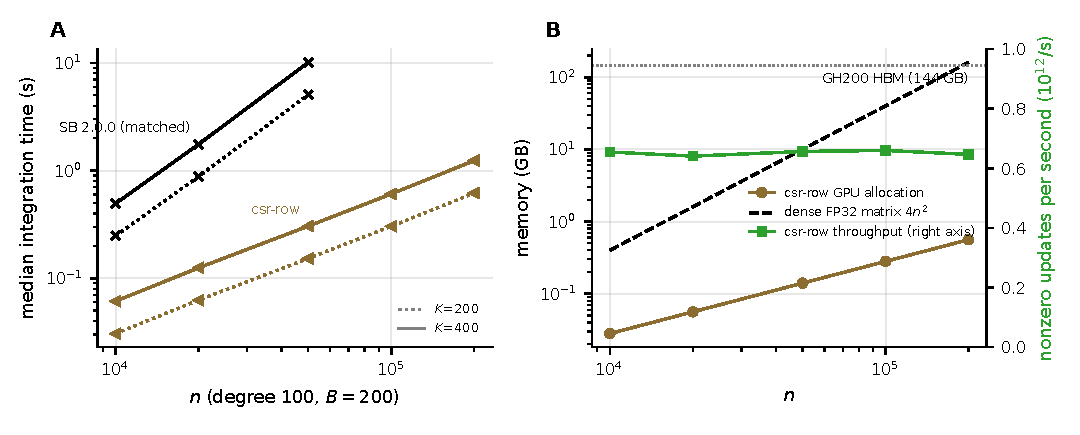
\includegraphics[width=\linewidth]{fig3_sparse_scaling.pdf}
\caption{Sparse scaling on regular bipartite graphs of degree 100 (\code{csr-row}, FP32, $B=200$, 10 trials, $\Delta t$ chosen per instance). Panel~A: median integration time against $n$ for $K=200$ and $K=400$; SB~2.0.0 (matched schedule) could be run only up to $n=50{,}000$. Panel~B: measured GPU allocation of the CSR path compared with the $4n^2$ bytes of a dense FP32 coupling matrix (left axis), and nonzero-update throughput $KB\,\mathrm{nnz}/T_{\mathrm{solve}}$ (right axis).}
\label{fig:sparse}
\end{figure}

\subsection{Dense scaling and capacity}\label{sec:res-dense}
Figure~\ref{fig:dense} reports the \code{gemm} path on dense random real-valued couplings with $n$ from 20,000 to 450,000, $K=50$, $B\in\{1,8,64\}$, against a PyTorch dense dSB implementation with the same state layout. The coupling matrix is placed in HBM while it fits within 0.85 of the free device memory; beyond that it is placed either entirely in the coherent Grace memory or with the HBM filled first and only the remaining rows in Grace memory (Section~\ref{sec:placement}). PyTorch can only use HBM. Four regimes appear.

\emph{Small matrices.} At $n=20{,}000$ the custom path is $1.9\times$ faster with FP16 operands and $1.4$--$4.3\times$ with FP32 storage (the larger factors at $B\ge8$ being TF32 against true FP32 in PyTorch).

\emph{HBM roofline.} From $n=80{,}000$ up to the HBM limit the FP16 paths coincide to within 9\% at $n=80{,}000$ and to within 3\% from $n=160{,}000$: both implementations move the whole $bn^2$-byte coupling matrix through HBM once per step at 4.2--4.3~TB/s, 86--88\% of the HBM3e peak of 4.9~TB/s, nearly independently of $B$ up to 64. In this regime the dense step is bandwidth-bound and there is nothing left for a kernel to gain; both implementations reach the roofline. The largest matrices held in HBM are $n=160{,}000$ in FP32 (102~GB) and $n=240{,}000$ in FP16 (115~GB), in agreement with the analytic limits of Table~\ref{tab:capacity}, and PyTorch fails to allocate beyond exactly these sizes.

\emph{Grace placement.} Beyond the HBM limit the custom path continues with the whole matrix in Grace memory: $n=200{,}000$--$300{,}000$ in FP32 (160--360~GB) and $n=300{,}000$--$450{,}000$ in FP16 (180--405~GB), where the PyTorch baseline runs out of memory at every size (Table~\ref{tab:grace}). The largest instance, $n=450{,}000$ in FP16, uses 67\% of the combined 601~GB budget. The step is bound by the link: the staged matrix is streamed at 371~GB/s at every size and in both operand formats (370.7--371.8~GB/s at $B=1$), 82\% of the nominal 450~GB/s per direction of NVLink-C2C and a factor of 11 below the HBM tier, so a step takes 0.43--0.97~s in FP32 and 0.49--1.09~s in FP16. Because the product on a staged block runs at the HBM rate, the serialisation of copy and product costs at most about 9\% of this time. The coupling matrix is read once per step for all replicas, so the step time is also independent of $B$: $B=64$ costs at most 2\% more than $B=1$ at every $n$, and 64 trajectories of a 450,000-variable dense instance advance at the price of one.

\emph{Hybrid placement.} Keeping the first rows in HBM removes 127~GB of every step's Grace traffic. The step time falls to 0.12, 0.31 and 0.66~s for FP32 at $n=200{,}000$, 240,000 and 300,000 (33, 103 and 233~GB streamed from Grace memory) and to 0.18, 0.56 and 0.78~s for FP16 at $n=300{,}000$, 400,000 and 450,000 (53, 193 and 278~GB), which is $3.65$, $2.02$ and $1.48\times$, respectively $2.72$, $1.55$ and $1.39\times$, faster than Grace placement. As Eq.~\eqref{eq:tier} predicts, the gain is largest just past the HBM limit and shrinks as the Grace share grows. With the two bandwidths measured in the pure placements, $BW_H=4.2$~TB/s and $BW_G=371$~GB/s, Eq.~\eqref{eq:tier} reproduces all six hybrid step times to within 4\% (within 1.2\% for five of them), so the split adds no measurable cost beyond the bytes it moves. The step time again depends only weakly on the batch size ($B=64$ within 6\% of $B=1$).

\begin{table}[!ht]\centering\small
\caption{Dense \code{gemm} beyond the HBM limit ($K=50$, median of three repetitions): whole matrix in Grace memory, and hybrid placement with the HBM filled first (``In Grace'' = part of the matrix streamed from Grace memory). GB/s is the coupling-matrix bandwidth $bn^2/T_{\mathrm{step}}$ at $B=1$; ``Speedup'' is the Grace-placement step time divided by the hybrid step time at $B=1$. The PyTorch baseline cannot allocate any of these matrices.}
\label{tab:grace}
\resizebox{\linewidth}{!}{% auto-generated: dsb-gpu gemm beyond the HBM limit, K=50, median of 3 repetitions; GB/s = bn^2/T_step at B=1
\begin{tabular}{lrrrrrrrrrr}\toprule
 & & & \multicolumn{3}{c}{Grace only} & \multicolumn{4}{c}{Hybrid HBM+Grace} & \\
\cmidrule(lr){4-6}\cmidrule(lr){7-10}
Operands & $n$ & Matrix (GB) & $B=1$ (s) & $B=64$ (s) & GB/s & In Grace (GB) & $B=1$ (s) & $B=64$ (s) & GB/s & Speedup\\\midrule
FP32 & 200{,}000 & 160 & 0.430 & 0.437 & 372 & 33 & 0.118 & 0.124 & 1359 & 3.65 \\
FP32 & 240{,}000 & 230 & 0.620 & 0.632 & 371 & 103 & 0.308 & 0.317 & 749 & 2.02 \\
FP32 & 300{,}000 & 360 & 0.971 & 0.990 & 371 & 233 & 0.658 & 0.673 & 547 & 1.48 \\
FP16 & 300{,}000 & 180 & 0.485 & 0.494 & 371 & 53 & 0.178 & 0.181 & 1009 & 2.72 \\
FP16 & 400{,}000 & 320 & 0.863 & 0.877 & 371 & 193 & 0.555 & 0.558 & 577 & 1.55 \\
FP16 & 450{,}000 & 405 & 1.090 & 1.107 & 371 & 278 & 0.783 & 0.791 & 517 & 1.39 \\
\bottomrule\end{tabular}
}
\end{table}

\begin{figure}[!ht]\centering
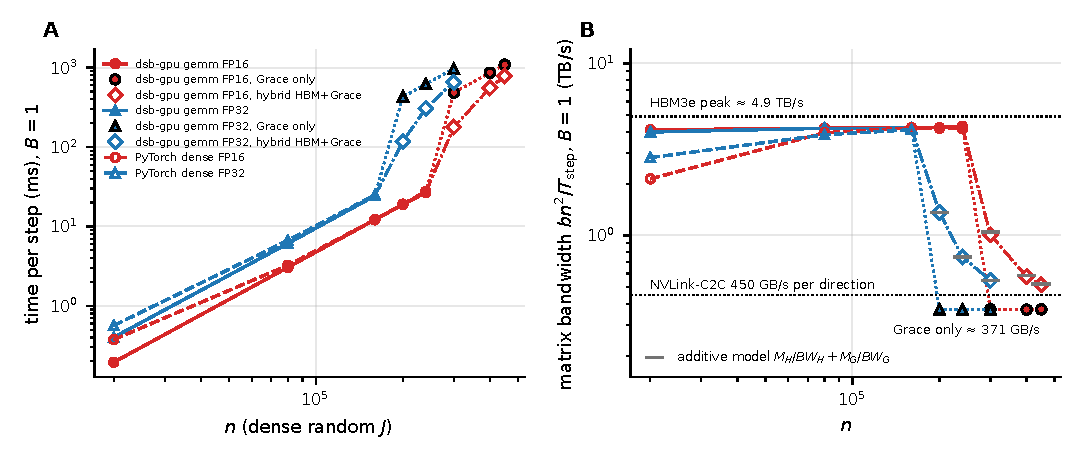
\includegraphics[width=\linewidth]{fig8_dense_scaling.pdf}
\caption{Dense scaling with random real-valued couplings ($K=50$, $B=1$, three repetitions). Filled markers: coupling matrix in HBM; black-edged markers joined by dotted lines: whole matrix in Grace memory; open diamonds joined by dash-dotted lines: hybrid placement with the HBM filled first. Panel~A: time per step against $n$ for the \code{gemm} path and a PyTorch dense dSB implementation, FP16 and FP32 operands (TF32 for \code{gemm}); PyTorch stops where HBM is exhausted (FP32: 160,000; FP16: 240,000). Panel~B: coupling-matrix bandwidth $bn^2/T_{\mathrm{step}}$: 4.2--4.3~TB/s in HBM for $n\ge 80{,}000$, 371~GB/s from Grace memory, and in between for the hybrid placement, where the grey ticks are the prediction of Eq.~\eqref{eq:tier} from the two measured bandwidths.}
\label{fig:dense}
\end{figure}

\subsection{Dense $\pm1$ couplings at one bit per coupling on two GH200s}\label{sec:res-bitmulti}
Table~\ref{tab:bitmulti} and Figure~\ref{fig:bitmulti} report \code{bit\_dense\_multi} (Section~\ref{sec:bitexact}) on random dense $\pm1$ couplings with $n$ from 500,000 to 3,000,000, $K=50$ and $B=1$, with the rows of the packed matrix divided between the two GH200s of the system. Up to $n=1{,}000{,}000$ the 125~GB matrix fits in the two HBMs (62.5~GB per GPU) and a step takes 13.9~ms: each GPU reads its half of the matrix at 4.49~TB/s, 92\% of the HBM3e peak, an aggregate of 8.97~TB/s. From $n=2{,}000{,}000$ each GPU fills its HBM budget of 127~GB and streams the remaining rows from its own Grace node---246, 527 and 871~GB in total at $n=2{,}000{,}000$, 2,500,000 and 3,000,000---and the step takes 0.41, 0.84 and 1.40~s. The largest matrix, 1.125~TB at $n=3{,}000{,}000$, occupies 94\% of the combined $2\times601$~GB budget of Table~\ref{tab:capacity}. Preparation, which generates and pins the matrix, takes 81~s at that size and is excluded from the step time as everywhere else in this paper.

Equation~\eqref{eq:tier}, with the aggregate bandwidths measured on this path---$BW_H=8.97$~TB/s from the HBM-resident points and $BW_G=646$~GB/s (323~GB/s per GPU) from the Grace share of the hybrid points---reproduces the three hybrid step times to within 2\% ($-0.4$, $0.0$ and $+1.9$\%). The per-GPU timing of one step at $n=3{,}000{,}000$ shows where the time goes: the HBM rows take 28.5~ms on either GPU (4.46~TB/s), the Grace rows 1373~ms on GPU~0 and 1236~ms on GPU~1 (317 and 352~GB/s; the two NUMA nodes are not identical, and the difference was not investigated), the update kernel 0.01~ms, and the exchange of the 375~KB sign bitmaps 0.10~ms, after which GPU~1 waits 138~ms for GPU~0. The step is therefore set by the slower of the two Grace links, and inter-GPU communication is negligible for this algorithm because the only quantity the GPUs share is the sign vector. The per-GPU Grace bandwidth is 87\% of the 371~GB/s measured for the single-GPU \code{gemm} path, the difference being the serialisation of each staged copy with the population-count kernel that consumes it.

The storage format is what moves the operating point. The largest dense instance of Section~\ref{sec:res-dense}, $n=450{,}000$ in FP16, holds $2.0\times10^{11}$ couplings in 405~GB and advances one step in 0.78~s on one GPU; at one bit per coupling the $n=3{,}000{,}000$ instance holds 44 times as many couplings in 1.125~TB and advances one step in 1.40~s on two GPUs, that is $25\times$ less time per coupling, or $12\times$ per GPU, against the sixteen-fold reduction in bytes per coupling (the remainder is the larger Grace share, 77\% against 69\% of the matrix). A 1000-step trajectory of the 3,000,000-variable instance takes 23 minutes.

The Mattis runs extend the bit-for-bit host check of Section~\ref{sec:bitexact}, which is limited to small $n$, to the full scale. For every $n$ and each of the three hidden solutions $\xi$, the final energy equals the planted ground-state energy $-n(n-1)/2$ exactly (15 of 15 runs; the final-state checksums differ between seeds, as they must), and the step time is within 0.3\% of that on the random instance of the same size, as expected for a kernel whose work does not depend on the coupling values. Since a Mattis instance is gauge-equivalent to a ferromagnet, this is a correctness statement about the two-GPU, two-tier data path---row staging, bitmap exchange and energy evaluation---and not evidence about the optimisation power of dSB on hard instances of this size.

\begin{table}[!ht]\centering\small
\caption{\code{bit\_dense\_multi} on two GH200s ($K=50$, $B=1$): dense $\pm1$ coupling matrix at one bit per coupling, rows split between the GPUs, each GPU filling its HBM first (``Split'') and streaming the remaining rows from its own Grace node. Random $\pm1$ instances: median step time of three repetitions and coupling-matrix bandwidth $n^2/8/T_{\mathrm{step}}$ summed over both GPUs. Mattis instances: number of hidden solutions (seeds 42--44) for which the final energy equals $-n(n-1)/2$, and the step time.}
\label{tab:bitmulti}
\resizebox{\linewidth}{!}{% auto-generated: bit_dense_multi, 2 GH200s, K=50, B=1; random +-1 J: median of 3 repetitions; Mattis: one run per seed, found = energy equals -n(n-1)/2
\begin{tabular}{rrlrrrrrr}\toprule
 & & & \multicolumn{2}{c}{Split (GB)} & \multicolumn{2}{c}{Random $\pm1$ $J$} & \multicolumn{2}{c}{Mattis} \\
\cmidrule(lr){4-5}\cmidrule(lr){6-7}\cmidrule(lr){8-9}
$n$ & Matrix (GB) & Placement & HBM & Grace & $T_{\mathrm{step}}$ (s) & GB/s & Found & $T_{\mathrm{step}}$ (s)\\\midrule
500{,}000 & 31 & HBM & 31 & 0 & 0.0035 & 8952 & 3/3 & 0.0035 \\
1{,}000{,}000 & 125 & HBM & 125 & 0 & 0.0139 & 8991 & 3/3 & 0.0139 \\
2{,}000{,}000 & 500 & HBM + Grace & 254 & 246 & 0.4069 & 1229 & 3/3 & 0.4073 \\
2{,}500{,}000 & 781 & HBM + Grace & 254 & 527 & 0.8436 & 926 & 3/3 & 0.8455 \\
3{,}000{,}000 & 1125 & HBM + Grace & 254 & 871 & 1.4015 & 803 & 3/3 & 1.4009 \\
\bottomrule\end{tabular}
}
\end{table}

\begin{figure}[!ht]\centering
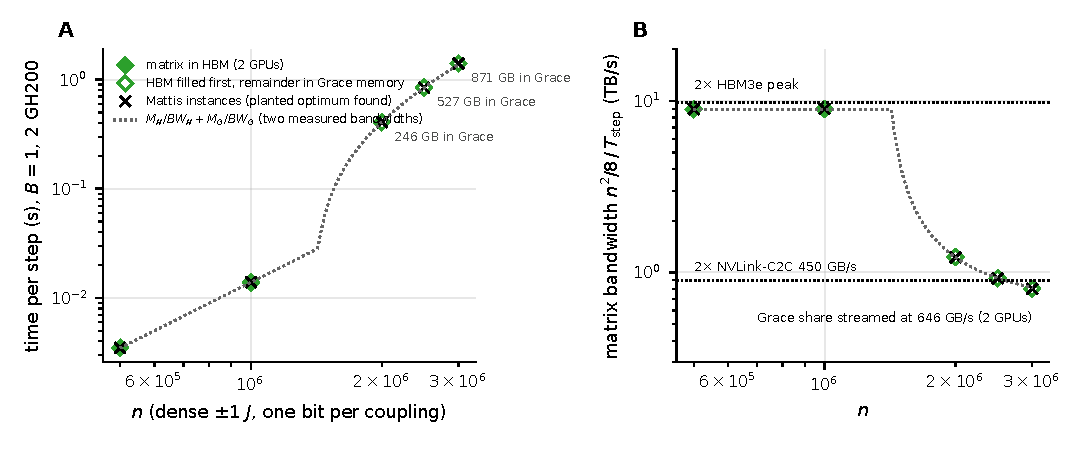
\includegraphics[width=\linewidth]{fig9_bit_multi.pdf}
\caption{Dense $\pm1$ bit path on two GH200s ($K=50$, $B=1$, three repetitions). Panel~A: time per step against $n$; filled diamonds: matrix in the two HBMs; open diamonds: each GPU's HBM filled first and the remaining rows (annotated) streamed from Grace memory; crosses: Mattis instances, all of which reached the planted optimum; dotted line: Eq.~\eqref{eq:tier} with the two aggregate bandwidths measured on this path. Panel~B: coupling-matrix bandwidth $n^2/8/T_{\mathrm{step}}$ summed over the two GPUs, against the aggregate HBM3e peak and NVLink-C2C rate.}
\label{fig:bitmulti}
\end{figure}

\FloatBarrier
\section{Discussion}\label{sec:discussion}
The measurements locate the practical value of each execution path more precisely than the design expectations did, and in two places differently.

The first concerns temporal fusion. It was introduced to remove launch and intermediate-state traffic, and it does remove them; but on a dense instance with hundreds of replicas those costs are small beside the coupling traffic, and the quantity that decides the comparison with the library path is the replica reuse depth of Eq.~\eqref{eq:intensity}. The shared-memory budget caps that depth at $S_{\max}/13n$ and the occupancy constraint caps it at $B/N_{\mathrm{SM}}$; at $B=512$ the second cap is three and the implementation ran with one, so the dense fused path carried no matrix reuse at all and was $29\times$ slower than the library path on K2000. The capacity ceiling of the fused kernel, roughly 25,800 variables in the $9n$-byte layout on this device, is often presented as its principal limitation; the binding limitation at practical batch sizes is different and more restrictive, and it is relieved only by batches of a thousand replicas or more. Where fusion pays decisively is the sparse case: the fused CSR kernels are the fastest path on 27 of the 36 benchmark instances---all ten G-set instances with average degree up to five and 17 of the 19 QPLIB instances---because there the per-step work is a few microseconds and a launch per step would dominate it. The benefit of fusion scales inversely with the work per step: it removes a fixed per-step cost, which is decisive when the product is cheap and negligible when a dense product of $n^2B$ multiply--accumulates dominates. The same inverse relation holds across batch sizes on one dense instance: on K2000 the fused \code{bit} kernel, which adds exactness and a sixteen- to thirty-two-fold smaller coupling footprint on top of fusion, is the fastest path at 64 replicas or fewer, where the graph-captured products are held at a floor of about 7~\textmu s per step by their per-step kernel boundaries, and falls behind the tensor-core products at 128 replicas and more, where the product dominates.

The second concerns precision. The usual framing treats reduced precision as a speed-for-accuracy exchange to be evaluated empirically. For ternary couplings that framing does not apply to the TF32, INT8 and bit-packed paths: they are not approximations, and there is nothing to trade. Two consequences follow. The default cuBLAS math mode on Hopper, TF32, can be used on Max-Cut and ternary QUBO instances without any accuracy argument, which a solver written for real-valued couplings would not be entitled to assume. And the one path that is faster than the exact group, FP16 operands, is faster by $2.2\times$ on the instances where the product dominates while producing a different but, in every objective distribution we measured, statistically indistinguishable trajectory. The genuine trade-off is therefore between an exact narrow path and an approximate narrower one; on the ternary instances measured here, surrendering the guarantee cost nothing measurable, but on weighted instances, where coupling magnitudes span a wider range and FP16 storage is no longer exact, the question is open and the four weighted QPLIB instances do not settle it.

The comparison with the public package needs the same care in both directions. The speedups on QPLIB and on the small G-set instances are large because the package spends about 170~\textmu s per step in host dispatch at these sizes; the corresponding $50$--$85\times$ ratios measure the elimination of that overhead by persistent kernels and graph capture, which is a real and reproducible advantage for a user of the package but not a statement about arithmetic throughput. On K2000 and the large G-set instances the package is compute-bound and the ratios of $13$--$137\times$ combine dense tensor-core arithmetic or sparse storage with the same dispatch saving. In the other direction, the package's own default schedule truncates the anneal at the budgets used here, and reporting only that comparison would have overstated the case by a further factor of about two in speed and considerably more in quality; the matched schedule is the fair reference, and the remaining quality difference on K2000 is small enough to be attributable to the two rows of Table~\ref{tab:align} that could not be aligned.

The comparison with published SB machines (Section~\ref{sec:res-literature}) adds a fourth observation. The FPGA machines of Goto et al.\ and Tatsumura et al.\ hold the coupling matrix on chip and complete one step of a single trial in 0.3--2.5~\textmu s, a latency that only the fused \code{bit} kernel at small batch approaches here (3.2~\textmu s for 16 trials); the GPU compensates by processing 512 replicas per step, so that each read of the coupling matrix serves hundreds of trials and the coupling-product throughput exceeds that of the 2048-spin FPGA design by nearly two orders of magnitude. Since TTS is the product of the time per step and the number of steps to solution, and the latter is a property of the dSB dynamics that neither platform changes, the shorter TTS of the present implementation on K2000, G1, G11 and G22 is a throughput result: at matched success probability the GPU finishes more trials per second. The same argument bounds the claim. On instances that are solved within a few hundred steps, the latency of a single-trial machine matters more than throughput, and on the large sparse G-set instances neither the present implementation nor the published single-GPU dSB reaches the best-known cut at the budgets used, so no TTS can be compared there.

The Grace tier adds a fifth observation. Unified memory is often presented as removing the capacity limit of a GPU; for dense dSB it does so, at a price that follows directly from the roofline of Section~\ref{sec:model} and that depends strongly on how the spilled matrix is placed. The dense step reads the whole coupling matrix once, so its time is the bytes held in each memory divided by the bandwidth at which that memory delivers them, Eq.~\eqref{eq:tier}. Pinned Grace memory streamed through an HBM staging buffer delivers 371~GB/s, 82\% of the nominal link rate; the first version of the Grace placement, which relied on driver-managed memory read in place, sustained only 80--91~GB/s, because page migration turned each streaming pass into fault-driven copies. Filling HBM first and streaming only the remainder then removes the HBM-resident share from the link traffic. Three consequences follow. First, the tier is useful for integration, not only for storage: a 405~GB FP16 matrix at $n=450{,}000$ advances one step in 0.78~s with hybrid placement, so a 1000-step FP16 trajectory takes 13 minutes on one GPU (3 minutes at $n=300{,}000$), where the PyTorch baseline cannot start. Second, since the step time does not depend on $B$, all the throughput available in this tier comes from replicas; a dense instance too large for HBM should be run with the largest batch the state arrays allow. Third, the step time is predictable from two measured bandwidths, so the remaining gains are also predictable: overlapping the staging copies with the products would save at most the $BW_G/BW_H\approx9\%$ of the step spent in the products, whereas the storage format acts on the dominant term directly. The dense $\pm1$ bit path of Section~\ref{sec:res-bitmulti} is the measured form of that statement: at one bit per coupling the same hybrid placement, applied on each of two GH200s, holds a 3,000,000-variable matrix (1.1~TB) and advances a step in 1.40~s, with the two-tier model again within 2\%, and the planted ground states of Mattis instances are recovered exactly at every size. The two-GPU part costs almost nothing for this algorithm, because the only quantity the GPUs must share per step is the sign bitmap, $n/8$ bytes, which takes 0.1~ms of a 1.4~s step; what the second GPU adds is a second HBM and a second Grace link, and the step is set by the slower of the two links.

\subsection{Limitations and threats to validity}
All runtimes are integration times; one-time preparation (tens of milliseconds per benchmark instance, up to 81~s of matrix generation and pinning for the largest two-GPU instance) is excluded on both sides. The alignment of Table~\ref{tab:align} is as complete as the package's interface allows; the gain normalisation and the intra-step order of operations differ, and quality differences of the size seen on K2000 cannot be separated from them. The FP16 and CSR paths are not bitwise identical to the exact group for reasons internal to their kernels that this study did not isolate; their quality is established statistically, on 50 trials per configuration. On the ten G-set instances with $n\ge5000$ neither implementation reaches the best-known cut within the budgets used, so the quality comparison there rests on gaps and no time to solution can be quoted; the single-V100 dSB of Goto et al.\ likewise reports best cuts below the best-known values on all ten after $10^{3}$--$10^{4}$~s of computation per instance (Table~S4 of \cite{goto2021}), which points to the dynamics rather than the implementation. The literature comparison of Section~\ref{sec:res-literature} is restricted to the instances and metrics that the published works report, at their operating points and ours; it crosses hardware generations and is not a controlled experiment. Comparison against one public dSB package establishes an implementation result relative to that package, not superiority over Max-Cut heuristics with strong local search \cite{benlic2013,dunning2018}. The regular bipartite scaling graphs are trivial for any solver and support only throughput and capacity claims. One GH200 system cannot establish portability across GPU generations; the \code{bit} and \code{block} paths depend on the 227~KB opt-in shared memory of Hopper, and Hopper-specific cluster results are identified as such. Beyond HBM the \code{gemm} path was run with FP32 and FP16 operands only; the INT8 format and the ternary bit-packed form, whose capacity advantages remain analytic in Table~\ref{tab:capacity}, were not run with the matrix in Grace memory, and the staging copies were not overlapped with the products. The dense-scaling instances are random real-valued or random $\pm1$ matrices used for throughput only, and the Mattis instances of Section~\ref{sec:res-bitmulti} are gauge-equivalent to a ferromagnet: reaching their planted optimum establishes that the two-GPU bit path integrates the dynamics correctly at 3,000,000 variables, not that dSB solves hard problems of that size. That path was run with one replica; a batched version, keeping the sign bitmap and the population counts per replica, would share each pass over the matrix among $B$ trajectories as the \code{gemm} path does, and was not implemented.

\section{Conclusion}\label{sec:conclusion}
We have described a GPU dSB implementation for the GH200 that executes the same discrete dynamics through temporally fused persistent kernels for dense, bit-packed and sparse couplings and through graph-captured library products, and evaluated the paths under one protocol against an aligned public baseline on K2000, 16 G-set and 19 QPLIB instances. For couplings in $\{-1,0,+1\}$ the integer and bit-packed coupling products are exact, and the TF32, FP32, INT8 and bit-packed paths were verified to return bitwise identical trajectories on every ternary instance, so their runtimes are comparable without a quality confound; the FP16 path is a further $2.2\times$ faster where the product dominates, at the price of that guarantee. The fastest path is decided by the coupling density and the batch size: the fused CSR kernels up to average degree about five, where they win on 27 of the 36 instances, tensor-core products above, with FP16 or INT8 operands, and on K2000 at 64 replicas or fewer the exact fused bit-packed kernel, at 3.2~\textmu s per step for 16 replicas; only the dense fused replica-tiled kernel is not competitive below about a thousand replicas because shared-memory capacity and occupancy cannot be satisfied together. At equal work the fastest path is $13.6\times$ faster than the aligned public package on K2000, $13.5$--$137\times$ on G-set and $18$--$86\times$ on QPLIB, while reaching the target at least as often on 35 of 36 instances; on the small instances most of this is the elimination of per-step dispatch, on the large ones it is arithmetic and storage. Under the time-to-solution definition of the SB literature, the implementation reaches the best-known cut of K2000 in 0.20~s, against 1.3~s and 1.7~s reported for a single-FPGA dSB machine and a single-V100 dSB, and its coupling-product throughput on that instance is $88\times$ that of the 2048-spin FPGA aSB design, the advantage being throughput over replicas rather than per-step latency. Sparse execution scales linearly to $10^7$ nonzeros at a constant $0.65\times10^{12}$ nonzero updates per second in under 600~MB, dense execution up to 240,000 variables runs at the HBM bandwidth roofline, and with the coupling matrix in Grace memory the same path runs dense instances of up to 450,000 variables (405~GB) that the PyTorch baseline cannot allocate, streaming the matrix at 371~GB/s, 82\% of the nominal NVLink-C2C rate, with a step time independent of the batch size; keeping as many rows as fit in HBM shortens that step by a further $1.4$--$3.7\times$, as predicted by an additive two-tier bandwidth model. A bit-packed path for dense $\pm1$ couplings applies the same placement on each of two GH200s and, at one bit per coupling, integrates 3,000,000-variable dense instances (1.1~TB of couplings) at 1.40~s per step with the sign bitmap as the only inter-GPU traffic, recovering the planted ground state of Mattis instances exactly at every size. The contribution is an implementation and evaluation study: no new dSB algorithm is proposed, and the region in which each execution path is preferable is reported as a measured map rather than a ranking.

\section*{Declarations}
\noindent\textbf{Code and data availability.} Repository, archived release, commit hash, input checksums, the per-trial records behind every table and figure, and the analysis scripts that produce them: [to be supplied]. Public benchmark sources are identified in the references.\par
\noindent\textbf{Funding, acknowledgments, author contributions, and competing interests.} [To be completed by the authors before submission.]

\appendix
\section{Notation}
\begin{table}[H]\centering\small
\caption{Symbols used in the performance model.}
\label{tab:notation}
\begin{tabular}{ll}\toprule
Symbol & Meaning \\
\midrule
$n$ & number of spin variables after standardisation \\
$B$ & number of independent replicas per launch \\
$K$ & number of integration steps \\
$R$ & replicas assigned to one thread block \\
$R_{\max}(n)$ & largest $R$ admitted by shared memory, Eq.~\eqref{eq:rmax} \\
$R_{\mathrm{eff}}$ & largest $R$ admitted by memory and occupancy, Eq.~\eqref{eq:reff} \\
$S_{\max}$ & opt-in shared memory per block, bytes \\
$N_{\mathrm{SM}}$ & streaming multiprocessors on the device \\
$b$ & bytes stored per coupling coefficient \\
$\beta$ & library tile extent along the replica dimension \\
$\rho$ & achieved replica reuse depth \\
$I$ & operations per coupling byte, Eq.~\eqref{eq:intensity} \\
$\hat p_B$ & estimated per-trial success probability ($P_S$ in \cite{goto2021}) \\
$r_{99}$ & restarts for 99\% success, Eq.~\eqref{eq:restarts} \\
$t$, $T_{\mathrm{com}}$ & integration time of one trial of $B$ replicas (computation time per batch in \cite{goto2021}) \\
$N_{\mathrm{step}}$, $N_{\mathrm{batch}}$ & $K$ and $B$ in the notation of \cite{goto2021} \\
$\delta$, $p_k$, $\xi$ & detuning, pump and coupling gain ($a_0$, $a(t_k)$, $c_0$ in \cite{goto2021}) \\
\bottomrule
\end{tabular}
\end{table}

\begin{thebibliography}{99}\small\setlength{\itemsep}{3pt}
\bibitem{lucas} A. Lucas, ``Ising formulations of many NP problems,'' \textit{Frontiers in Physics}, vol. 2, art. 5, 2014. \url{https://doi.org/10.3389/fphy.2014.00005}.
\bibitem{glover} F. Glover, G. Kochenberger, and Y. Du, ``A tutorial on formulating and using QUBO models,'' arXiv:1811.11538, 2018. \url{https://arxiv.org/abs/1811.11538}.
\bibitem{boros} E. Boros and P. L. Hammer, ``Pseudo-Boolean optimization,'' \textit{Discrete Applied Mathematics}, vol. 123, pp. 155--225, 2002. \url{https://doi.org/10.1016/S0166-218X(01)00341-9}.
\bibitem{kirkpatrick} S. Kirkpatrick, C. D. Gelatt, Jr., and M. P. Vecchi, ``Optimization by simulated annealing,'' \textit{Science}, vol. 220, pp. 671--680, 1983. \url{https://doi.org/10.1126/science.220.4598.671}.
\bibitem{goto2019} H. Goto, K. Tatsumura, and A. R. Dixon, ``Combinatorial optimization by simulating adiabatic bifurcations in nonlinear Hamiltonian systems,'' \textit{Science Advances}, vol. 5, no. 4, eaav2372, 2019. \url{https://doi.org/10.1126/sciadv.aav2372}.
\bibitem{goto2021} H. Goto, K. Endo, M. Suzuki, Y. Sakai, T. Kanao, Y. Hamakawa, R. Hidaka, M. Yamasaki, and K. Tatsumura, ``High-performance combinatorial optimization based on classical mechanics,'' \textit{Science Advances}, vol. 7, no. 6, eabe7953, 2021. \url{https://doi.org/10.1126/sciadv.abe7953}.
\bibitem{goto2016} H. Goto, ``Bifurcation-based adiabatic quantum computation with a nonlinear oscillator network,'' \textit{Scientific Reports}, vol. 6, art. 21686, 2016. \url{https://doi.org/10.1038/srep21686}.
\bibitem{kanao2022} T. Kanao and H. Goto, ``Simulated bifurcation assisted by thermal fluctuation,'' \textit{Communications Physics}, vol. 5, art. 153, 2022. \url{https://doi.org/10.1038/s42005-022-00929-9}.
\bibitem{kanao2023} T. Kanao and H. Goto, ``Simulated bifurcation for higher-order cost functions,'' \textit{Applied Physics Express}, vol. 16, art. 014501, 2023. \url{https://doi.org/10.35848/1882-0786/acaba9}.
\bibitem{tabu2026} X.-Z. Tao, Q.-G. Zeng, Z.-J. Huang, B.-W. Zuo, Y.-Q. Liu, J. Zhuang, H. Okawa, and M.-H. Yung, ``Tabu-Enhanced Simulated Bifurcation for combinatorial optimization,'' \textit{Communications Physics}, 2026. \url{https://doi.org/10.1038/s42005-026-02538-2}.
\bibitem{zeng2024} Q.-G. Zeng, X.-P. Cui, B. Liu, Y. Wang, P. Mosharev, and M.-H. Yung, ``Performance of quantum annealing inspired algorithms for combinatorial optimization problems,'' \textit{Communications Physics}, vol. 7, art. 249, 2024. \url{https://doi.org/10.1038/s42005-024-01705-7}.
\bibitem{sbqa2026} J. Paw{\l}owski, P. Tarasiuk, J. Tuziemski, {\L}. Pawela, and B. Gardas, ``Simulated Bifurcation Quantum Annealing,'' arXiv:2604.01050, 2026, preprint. \url{https://arxiv.org/abs/2604.01050}.
\bibitem{fpga2019} K. Tatsumura, A. R. Dixon, and H. Goto, ``FPGA-based simulated bifurcation machine,'' in \textit{International Conference on Field Programmable Logic and Applications (FPL)}, pp. 59--66, 2019. \url{https://doi.org/10.1109/FPL.2019.00019}.
\bibitem{tatsumura2021heart} K. Tatsumura, ``Large-scale combinatorial optimization in real-time systems by FPGA-based accelerators for simulated bifurcation,'' in \textit{Proceedings of the 11th International Symposium on Highly Efficient Accelerators and Reconfigurable Technologies (HEART)}, pp. 1--6, 2021. \url{https://doi.org/10.1145/3468044.3468045}.
\bibitem{tatsumura2021} K. Tatsumura, M. Yamasaki, and H. Goto, ``Scaling out Ising machines using a multi-chip architecture for simulated bifurcation,'' \textit{Nature Electronics}, vol. 4, pp. 208--217, 2021. \url{https://doi.org/10.1038/s41928-021-00546-4}.
\bibitem{mohseni2022} N. Mohseni, P. L. McMahon, and T. Byrnes, ``Ising machines as hardware solvers of combinatorial optimization problems,'' \textit{Nature Reviews Physics}, vol. 4, pp. 363--379, 2022. \url{https://doi.org/10.1038/s42254-022-00440-8}.
\bibitem{aramon2019} M. Aramon, G. Rosenberg, E. Valiante, T. Miyazawa, H. Tamura, and H. G. Katzgraber, ``Physics-inspired optimization for quadratic unconstrained problems using a digital annealer,'' \textit{Frontiers in Physics}, vol. 7, art. 48, 2019. \url{https://doi.org/10.3389/fphy.2019.00048}.
\bibitem{gonul2025} Y. E. Gonul, C. E. Kayan, I. Mustafazade, N. Kandasamy, and B. Taskin, ``GPU-accelerated simulated oscillator Ising/Potts machine solving combinatorial optimization problems,'' in \textit{Proceedings of the Great Lakes Symposium on VLSI (GLSVLSI)}, pp. 112--117, 2025. \url{https://doi.org/10.1145/3716368.3735247}.
\bibitem{vamsi2025} N. K. Vamsi, A. K. Singh, and A. Prabhakar, ``GPU-based digital annealing for accelerating large-scale combinatorial optimization,'' in \textit{2025 Supercomputing India (SCI)}, pp. 1--8, 2025. \url{https://doi.org/10.1109/SCI68648.2025.11333858}.
\bibitem{publicsb} R. Ageron, T. Bouquet, and L. Pugliese, \textit{Simulated Bifurcation algorithm for Python}, software repository. \url{https://github.com/bqth29/simulated-bifurcation-algorithm}. Experimental package pin: version 2.0.0. Accessed September 21, 2026.
\bibitem{pytorch} A. Paszke et al., ``PyTorch: An imperative style, high-performance deep learning library,'' in \textit{Advances in Neural Information Processing Systems}, vol. 32, 2019. \url{https://arxiv.org/abs/1912.01703}.
\bibitem{fasthare} P. Thai, M. T. Thai, T. Vu, and T. N. Dinh, ``FastHare: Fast Hamiltonian Reduction for Large-scale Quantum Annealing,'' \textit{IEEE International Conference on Quantum Computing and Engineering (QCE)}, pp. 114--124, 2022. \url{https://doi.org/10.1109/QCE53715.2022.00030}.
\bibitem{mao2026} C. Mao, P. Mosharev, Y. Wang, and M.-H. Yung, ``A reduction scheme for general-order Ising-like Hamiltonians in quantum heuristic solvers,'' arXiv:2607.19871, 2026, preprint. \url{https://arxiv.org/abs/2607.19871}.
\bibitem{roofline} S. Williams, A. Waterman, and D. Patterson, \textit{Roofline: An Insightful Visual Performance Model for Floating-Point Programs and Multicore Architectures}, Technical Report UCB/EECS-2008-134, University of California, Berkeley, 2008. \url{https://www2.eecs.berkeley.edu/Pubs/TechRpts/2008/EECS-2008-134.html}.
\bibitem{bell2009} N. Bell and M. Garland, ``Implementing sparse matrix-vector multiplication on throughput-oriented processors,'' in \textit{ACM/IEEE Conference on Supercomputing (SC)}, 2009. \url{https://doi.org/10.1145/1654059.1654078}.
\bibitem{yang2018} C. Yang, A. Bulu\c{c}, and J. D. Owens, ``Design principles for sparse matrix multiplication on the GPU,'' in \textit{Euro-Par 2018: Parallel Processing}, Lecture Notes in Computer Science, pp. 672--687, 2018. \url{https://doi.org/10.1007/978-3-319-96983-1_48}.
\bibitem{cuda} NVIDIA, \textit{CUDA Programming Guide}, CUDA Graphs and execution model documentation. \url{https://docs.nvidia.com/cuda/cuda-programming-guide/}. Accessed September 21, 2026.
\bibitem{cublas} NVIDIA, \textit{cuBLAS Library Documentation}, GEMM interfaces, computation types, and graph support. \url{https://docs.nvidia.com/cuda/cublas/}. Accessed September 21, 2026.
\bibitem{hopper} NVIDIA, \textit{Hopper Tuning Guide}, shared memory, occupancy, and thread-block clusters. \url{https://docs.nvidia.com/cuda/hopper-tuning-guide/}. Accessed September 21, 2026.
\bibitem{ronnow} T. F. R{\o}nnow, Z. Wang, J. Job, S. Boixo, S. V. Isakov, D. Wecker, J. M. Martinis, D. A. Lidar, and M. Troyer, ``Defining and detecting quantum speedup,'' \textit{Science}, vol. 345, pp. 420--424, 2014. \url{https://doi.org/10.1126/science.1252319}.
\bibitem{isakov2015} S. V. Isakov, I. N. Zintchenko, T. F. R\o nnow, and M. Troyer, ``Optimized simulated annealing for Ising spin glasses,'' \textit{Computer Physics Communications}, vol. 192, pp. 265--271, 2015. \url{https://doi.org/10.1016/j.cpc.2015.02.015}.
\bibitem{dolan2002} E. D. Dolan and J. J. Mor\'e, ``Benchmarking optimization software with performance profiles,'' \textit{Mathematical Programming}, vol. 91, pp. 201--213, 2002. \url{https://doi.org/10.1007/s101070100263}.
\bibitem{dunning2018} I. Dunning, S. Gupta, and J. Silberholz, ``What works best when? A systematic evaluation of heuristics for Max-Cut and QUBO,'' \textit{INFORMS Journal on Computing}, vol. 30, no. 3, pp. 608--624, 2018. \url{https://doi.org/10.1287/ijoc.2017.0798}.
\bibitem{benlic2013} U. Benlic and J.-K. Hao, ``Breakout local search for the Max-Cut problem,'' \textit{Engineering Applications of Artificial Intelligence}, vol. 26, no. 3, pp. 1162--1173, 2013. \url{https://doi.org/10.1016/j.engappai.2012.09.001}.
\bibitem{markidis2018} S. Markidis, S. W. D. Chien, E. Laure, I. B. Peng, and J. S. Vetter, ``NVIDIA tensor core programmability, performance \& precision,'' in \textit{IEEE International Parallel and Distributed Processing Symposium Workshops (IPDPSW)}, pp. 522--531, 2018. \url{https://doi.org/10.1109/IPDPSW.2018.00091}.
\bibitem{haidar2018} A. Haidar, S. Tomov, J. Dongarra, and N. J. Higham, ``Harnessing GPU tensor cores for fast FP16 arithmetic to speed up mixed-precision iterative refinement solvers,'' in \textit{SC18: International Conference for High Performance Computing, Networking, Storage and Analysis}, pp. 603--613, 2018. \url{https://doi.org/10.1109/SC.2018.00050}.
\bibitem{luo2024} W. Luo, R. Fan, Z. Li, D. Du, Q. Wang, and X. Chu, ``Benchmarking and dissecting the Nvidia Hopper GPU architecture,'' arXiv:2402.13499, 2024. \url{https://arxiv.org/abs/2402.13499}.
\bibitem{li2019bstc} A. Li, T. Geng, T. Wang, M. Herbordt, S. L. Song, and K. Barker, ``BSTC: A novel binarized-soft-tensor-core design for accelerating bit-based approximated neural nets,'' in \textit{Proceedings of the International Conference for High Performance Computing, Networking, Storage and Analysis (SC)}, pp. 1--30, 2019. \url{https://doi.org/10.1145/3295500.3356169}.
\bibitem{li2021bittc} A. Li and S. M. Su, ``Accelerating binarized neural networks via bit-tensor-cores in Turing GPUs,'' \textit{IEEE Transactions on Parallel and Distributed Systems}, vol. 32, no. 7, pp. 1878--1891, 2021. \url{https://doi.org/10.1109/TPDS.2020.3045828}.
\bibitem{simakov2024} N. A. Simakov, M. D. Jones, T. R. Furlani, E. Siegmann, and R. J. Harrison, ``First impressions of the NVIDIA Grace CPU Superchip and NVIDIA Grace Hopper Superchip for scientific workloads,'' in \textit{Proceedings of the International Conference on High Performance Computing in Asia-Pacific Region Workshops (HPC Asia Workshops)}, pp. 36--44, 2024. \url{https://doi.org/10.1145/3636480.3637097}.
\bibitem{bagchi2026} S. Bagchi, S. Srivastava, R. Levine, T. Sorensen, R. Stutsman, and V. Nagarajan, ``Consistency and coherence of the NVIDIA Grace-Hopper Superchip,'' in \textit{Proceedings of the 2026 ACM SIGPLAN International Symposium on Memory Management (ISMM)}, pp. 66--79, 2026. \url{https://doi.org/10.1145/3814942.3816134}.
\bibitem{qplib} F. Furini, E. Traversi, P. Belotti, A. Frangioni, A. Gleixner, N. Gould, L. Liberti, A. Lodi, R. Misener, H. Mittelmann, N. Sahinidis, S. Vigerske, and A. Wiegele, ``QPLIB: a library of quadratic programming instances,'' \textit{Mathematical Programming Computation}, vol. 11, pp. 237--265, 2019. \url{https://doi.org/10.1007/s12532-018-0147-4}. Instance repository: \url{https://qplib.zib.de/}.
\bibitem{gset} Y. Ye, \textit{G-set benchmark instance repository}, Stanford University. \url{https://web.stanford.edu/~yyye/yyye/Gset/}. Accessed September 21, 2026.
\end{thebibliography}
\end{document}
